\section{Introduction}

\hidenum
\begin{frame}[noframenumbering]
\frametitle{Contents}
 \tableofcontents[currentsection,hideothersubsections,sectionstyle=show/hide]
\end{frame}
\shownum

\subsection{Quick Overview of Parallel Hardware}

\begin{frame}
\begin{block}{Three Basic Flavors of Hardware}
    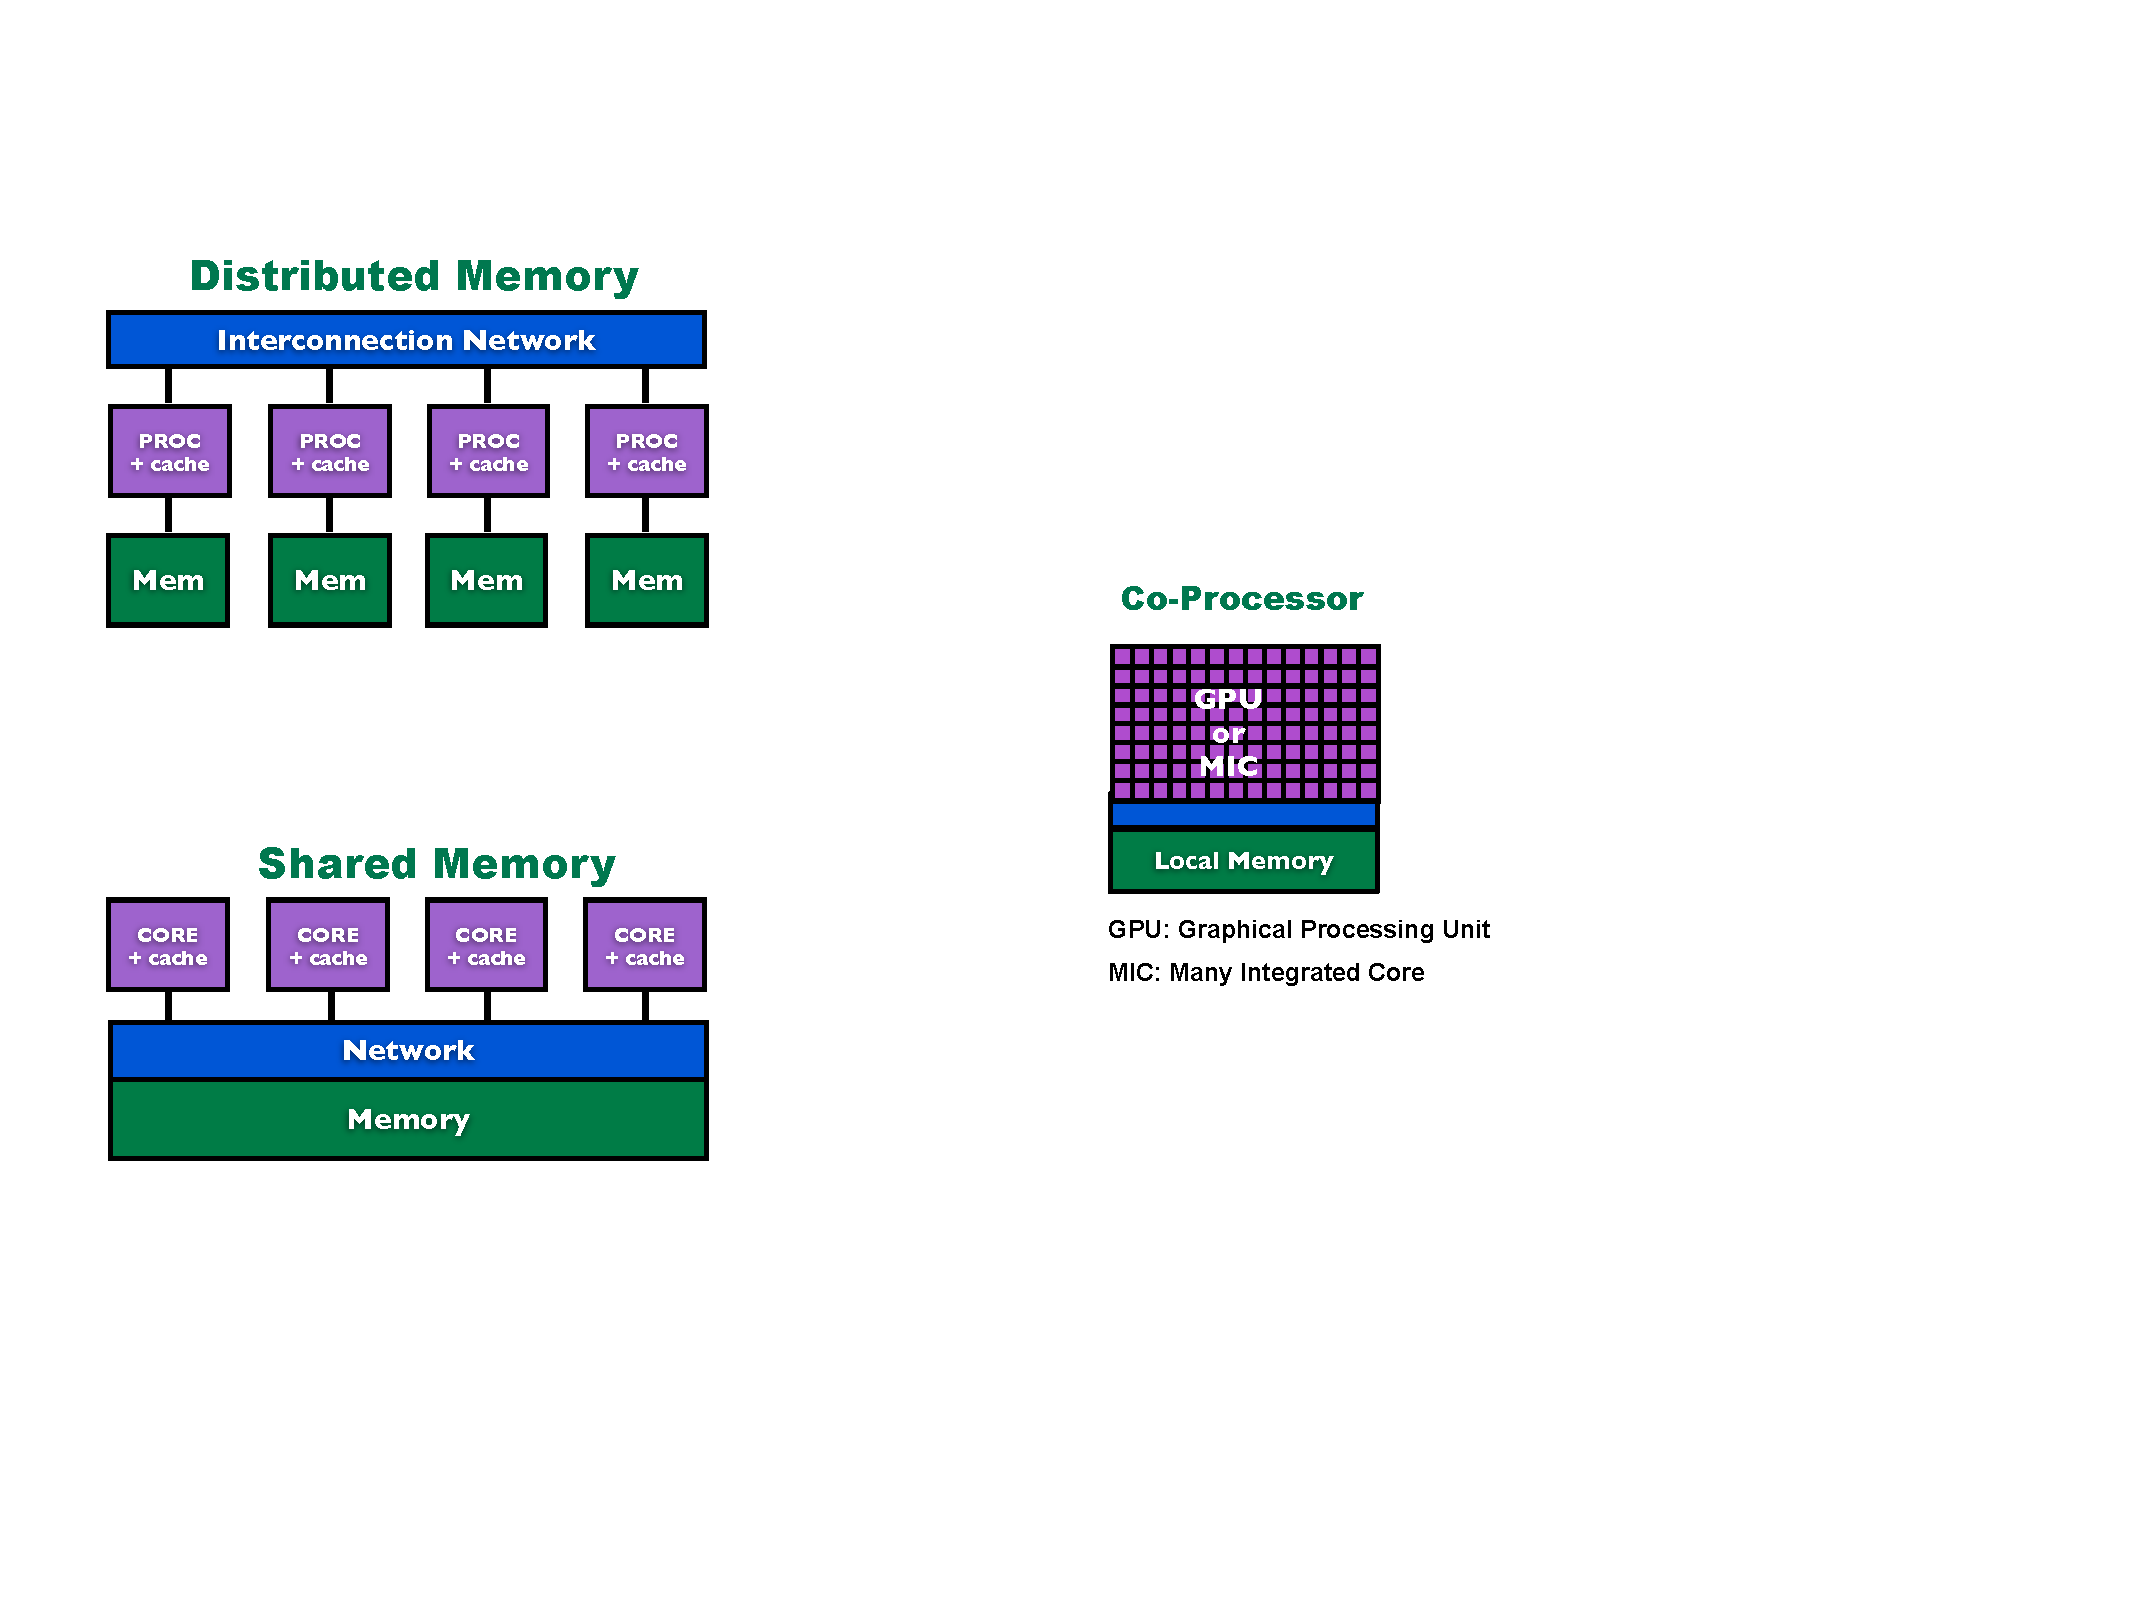
\includegraphics[width=0.95\textwidth]{pics/ParallelHardware1.pdf}
\end{block}
\end{frame}

\begin{frame}
\begin{block}{Your Laptop or Desktop}
    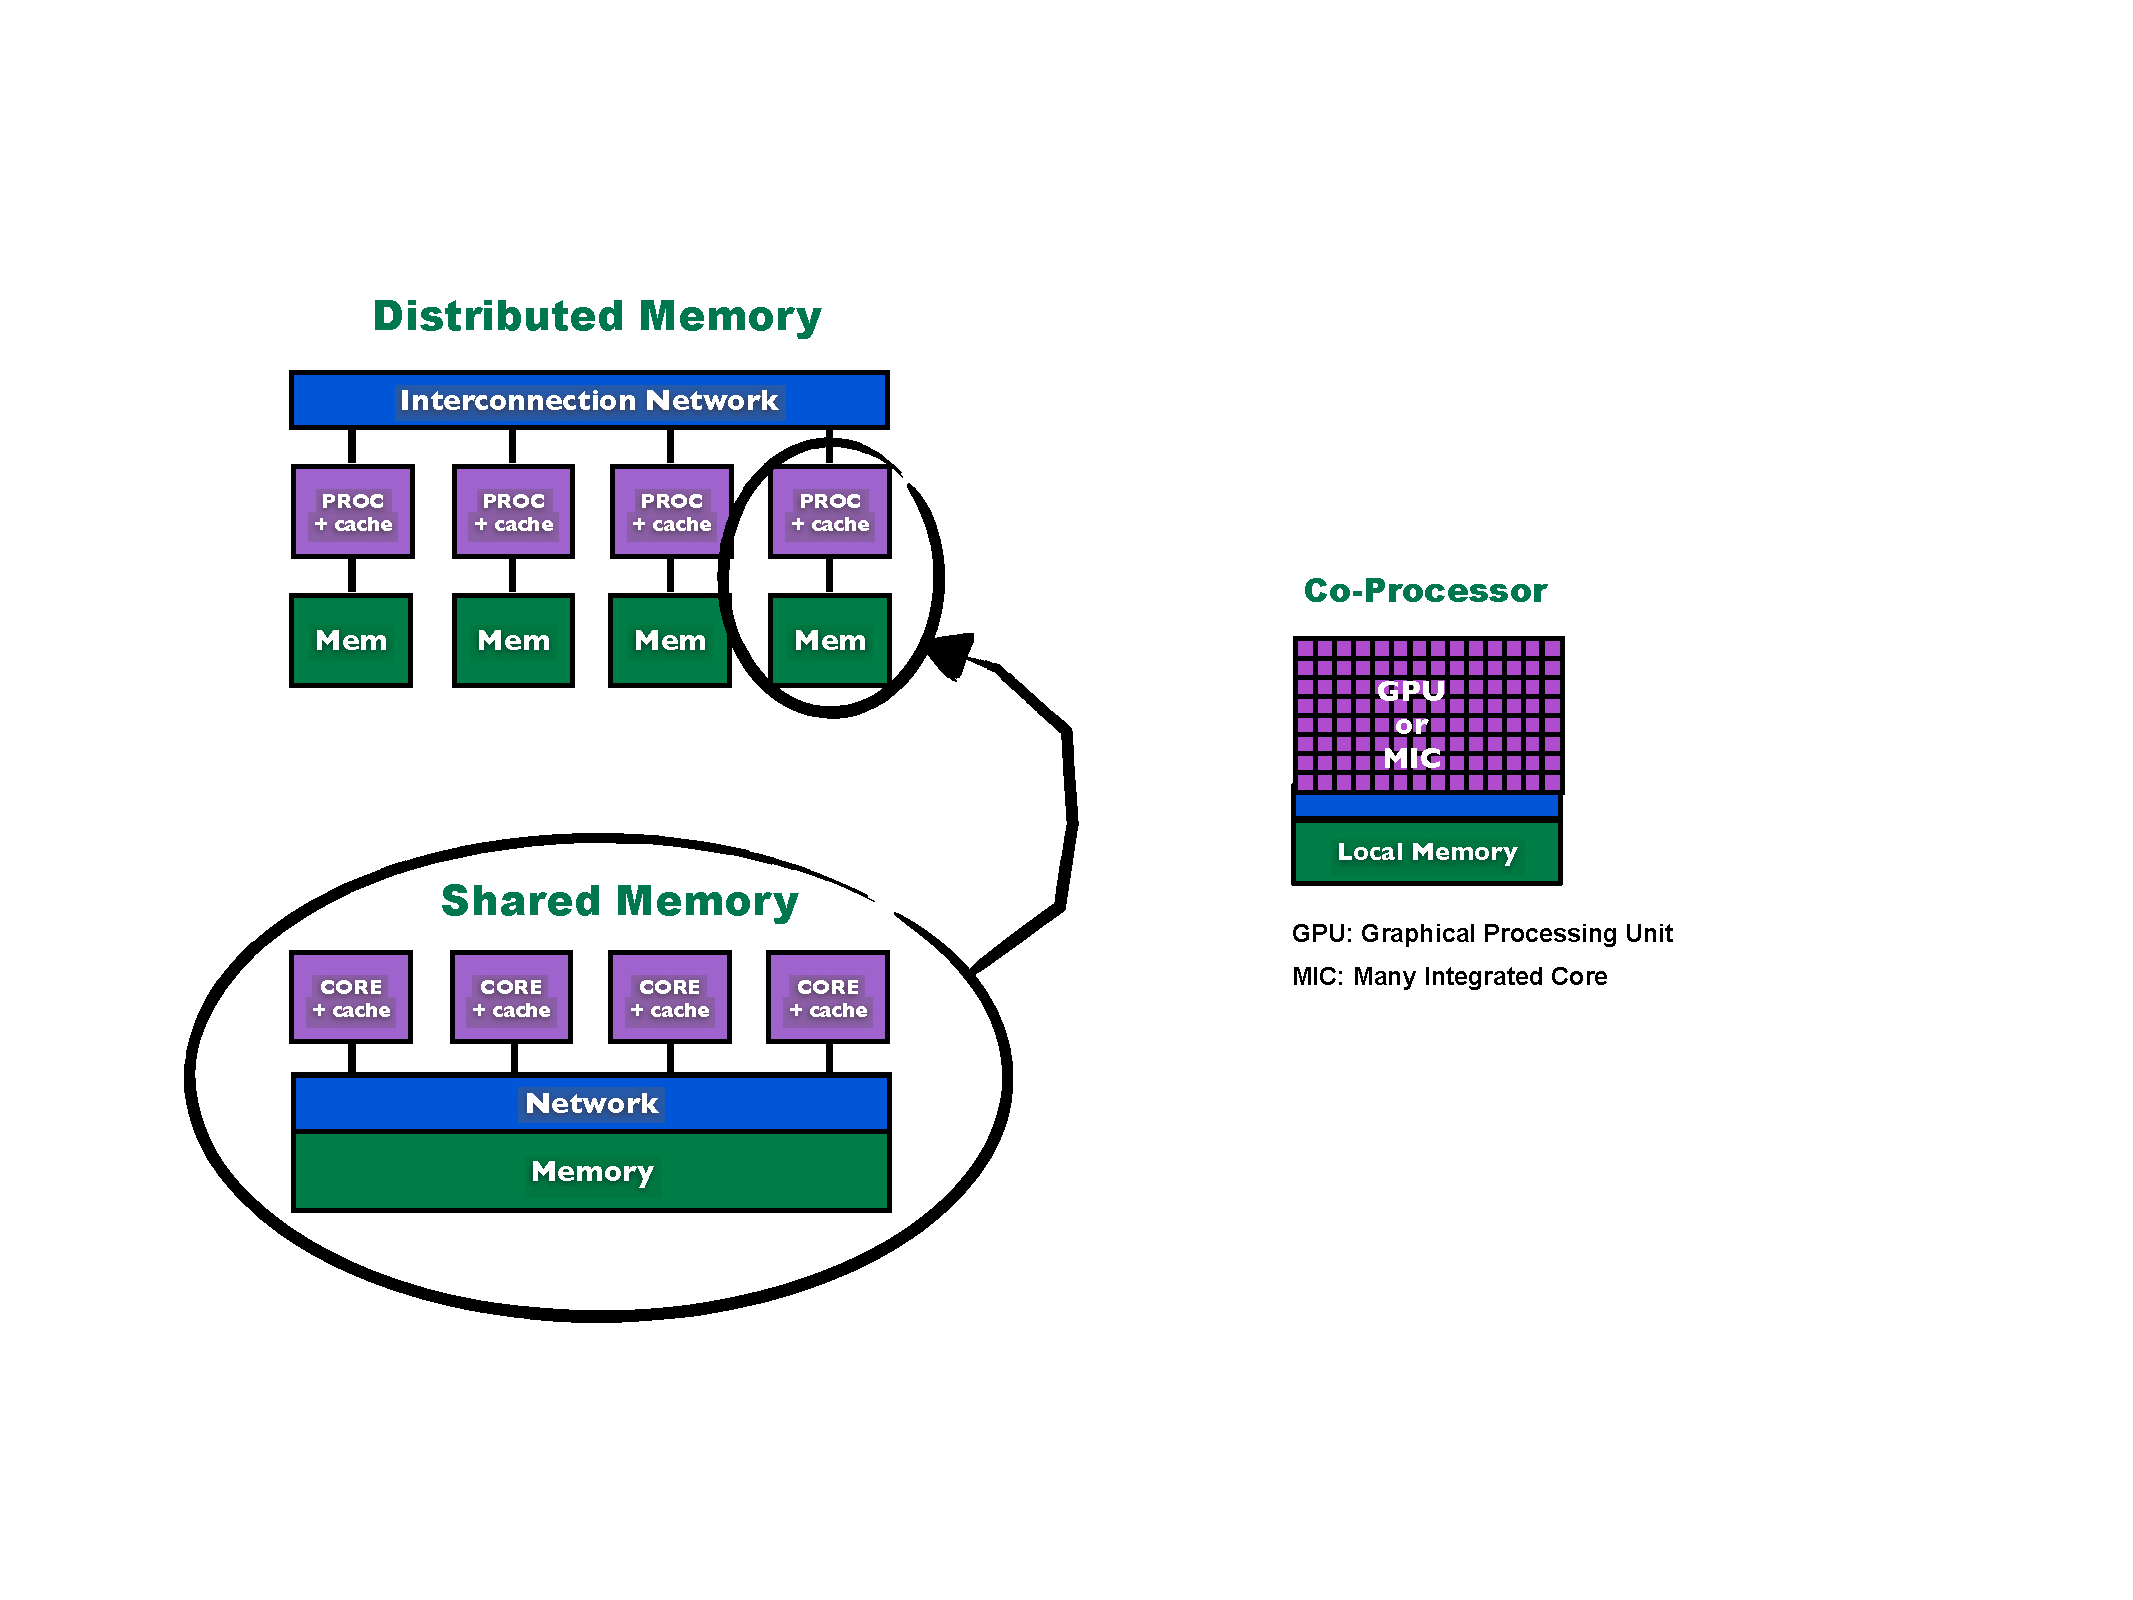
\includegraphics[width=0.95\textwidth]{pics/ParallelHardware2.pdf}
\end{block}
\end{frame}

\begin{frame}
\begin{block}{A Server or Cluster}
    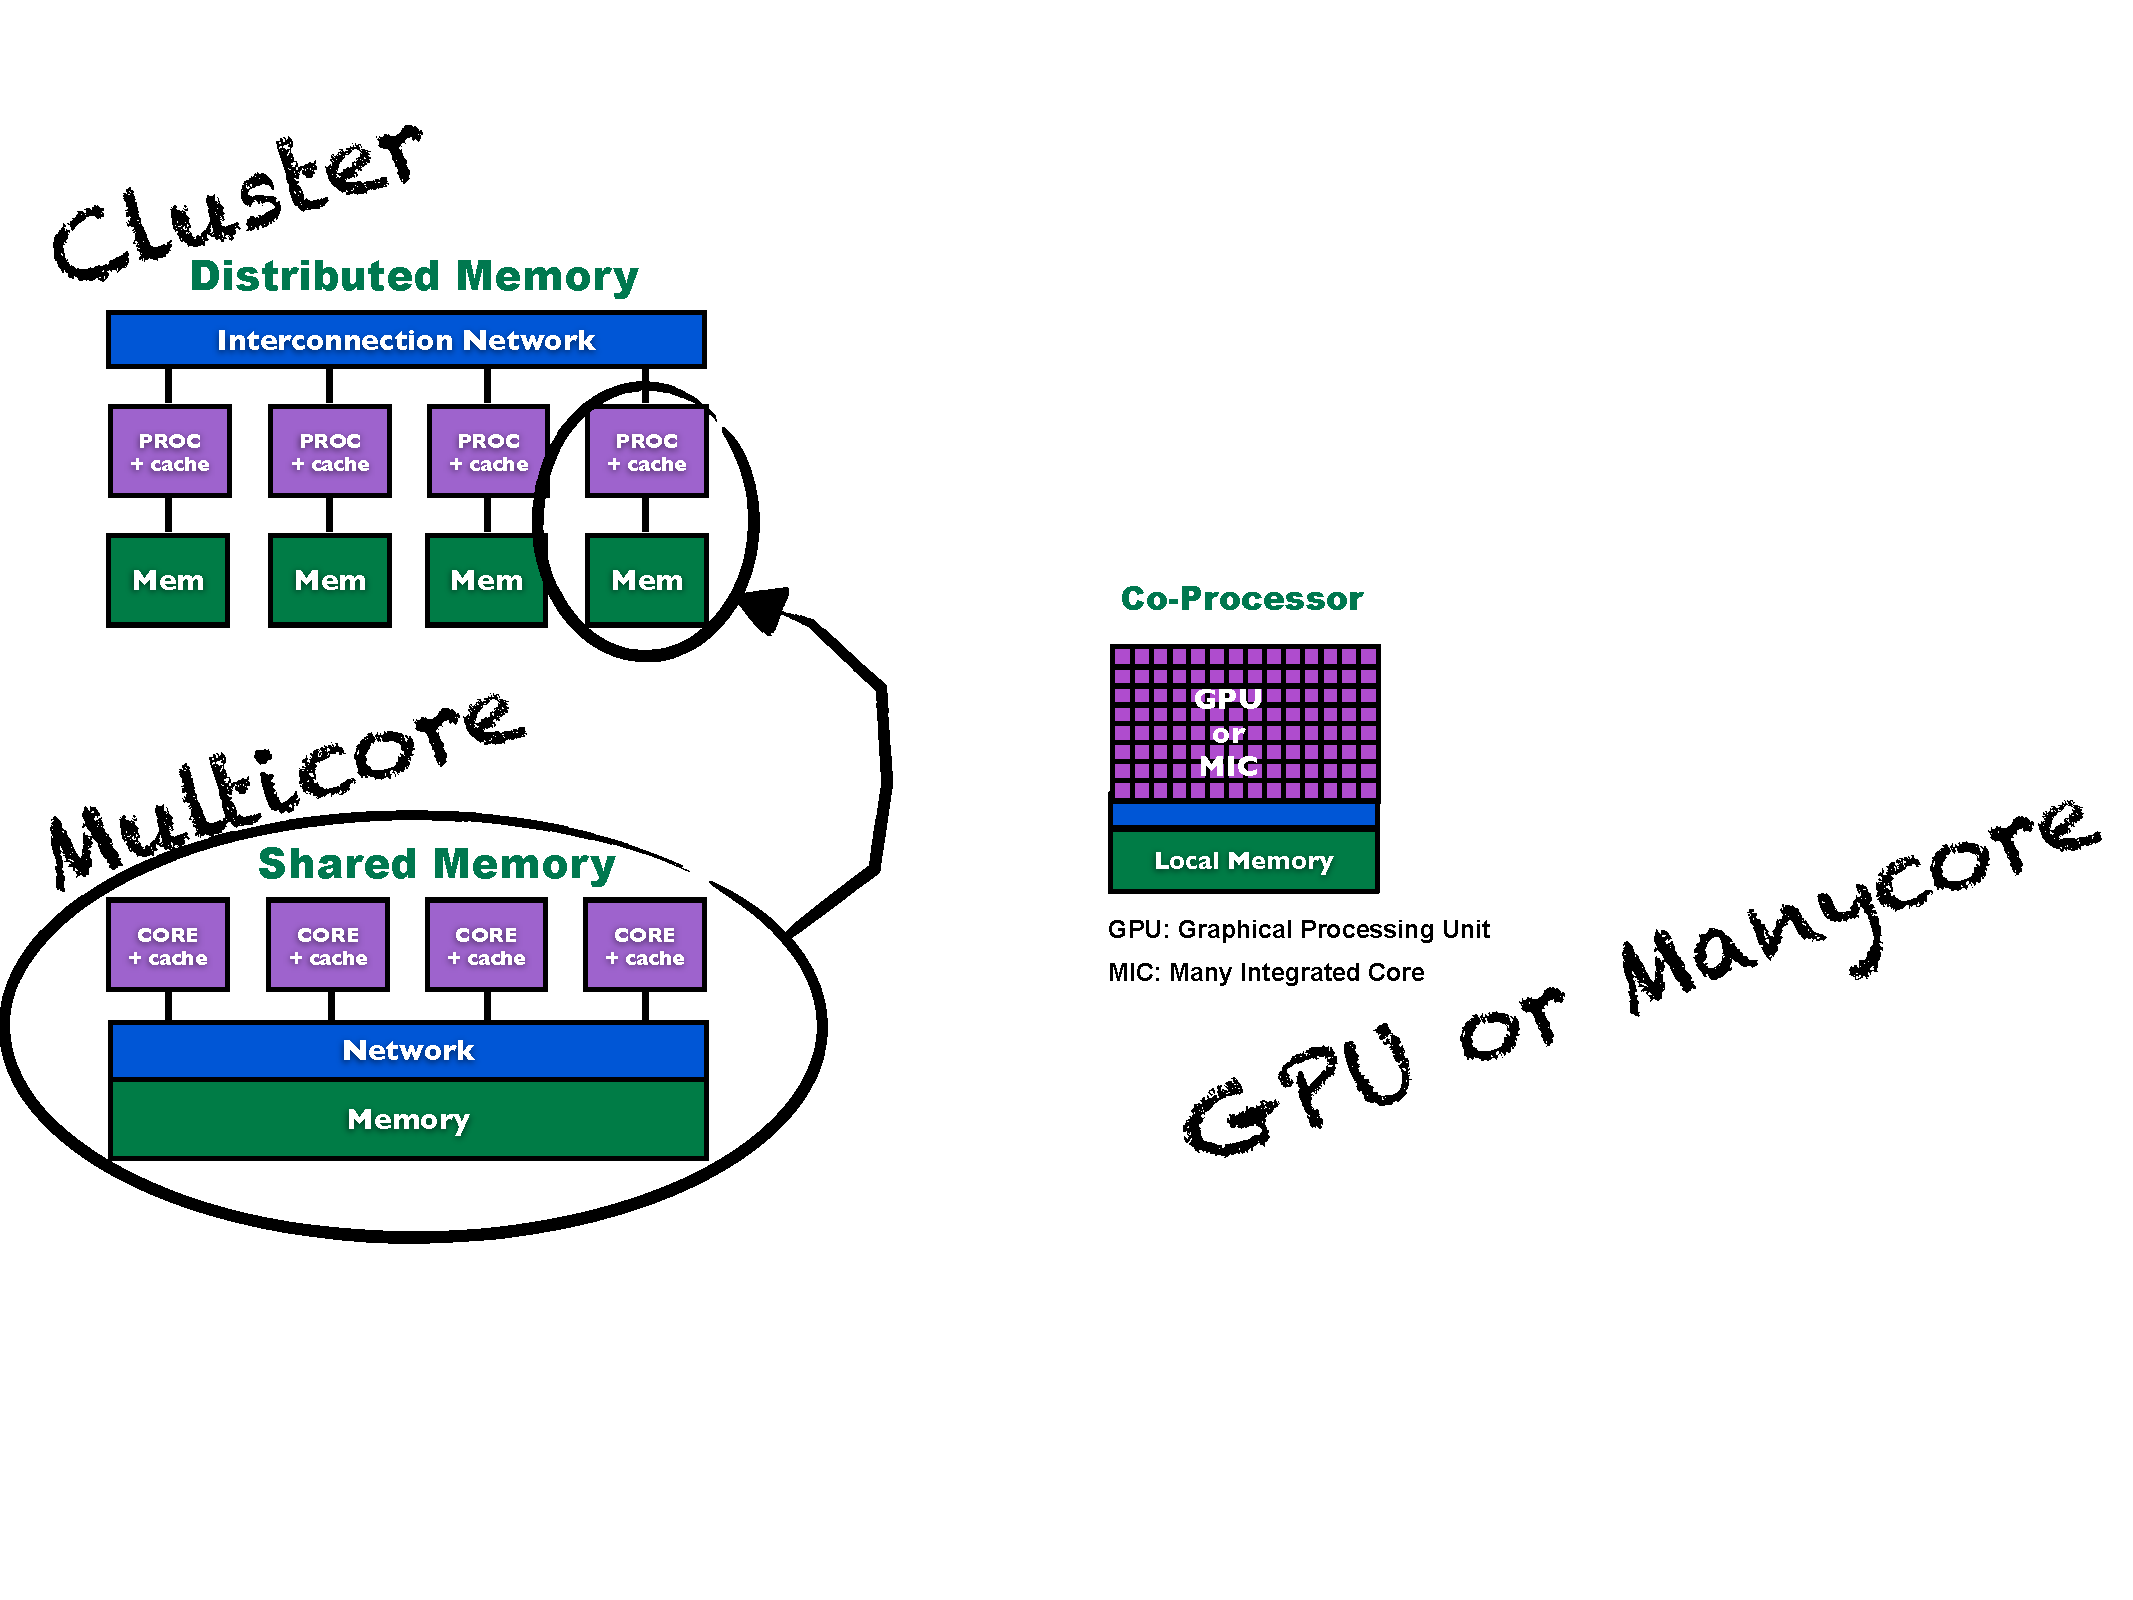
\includegraphics[width=0.95\textwidth]{pics/ParallelHardware3.pdf}
\end{block}
\end{frame}

\begin{frame}
\begin{block}{Server to Supercomputer}
    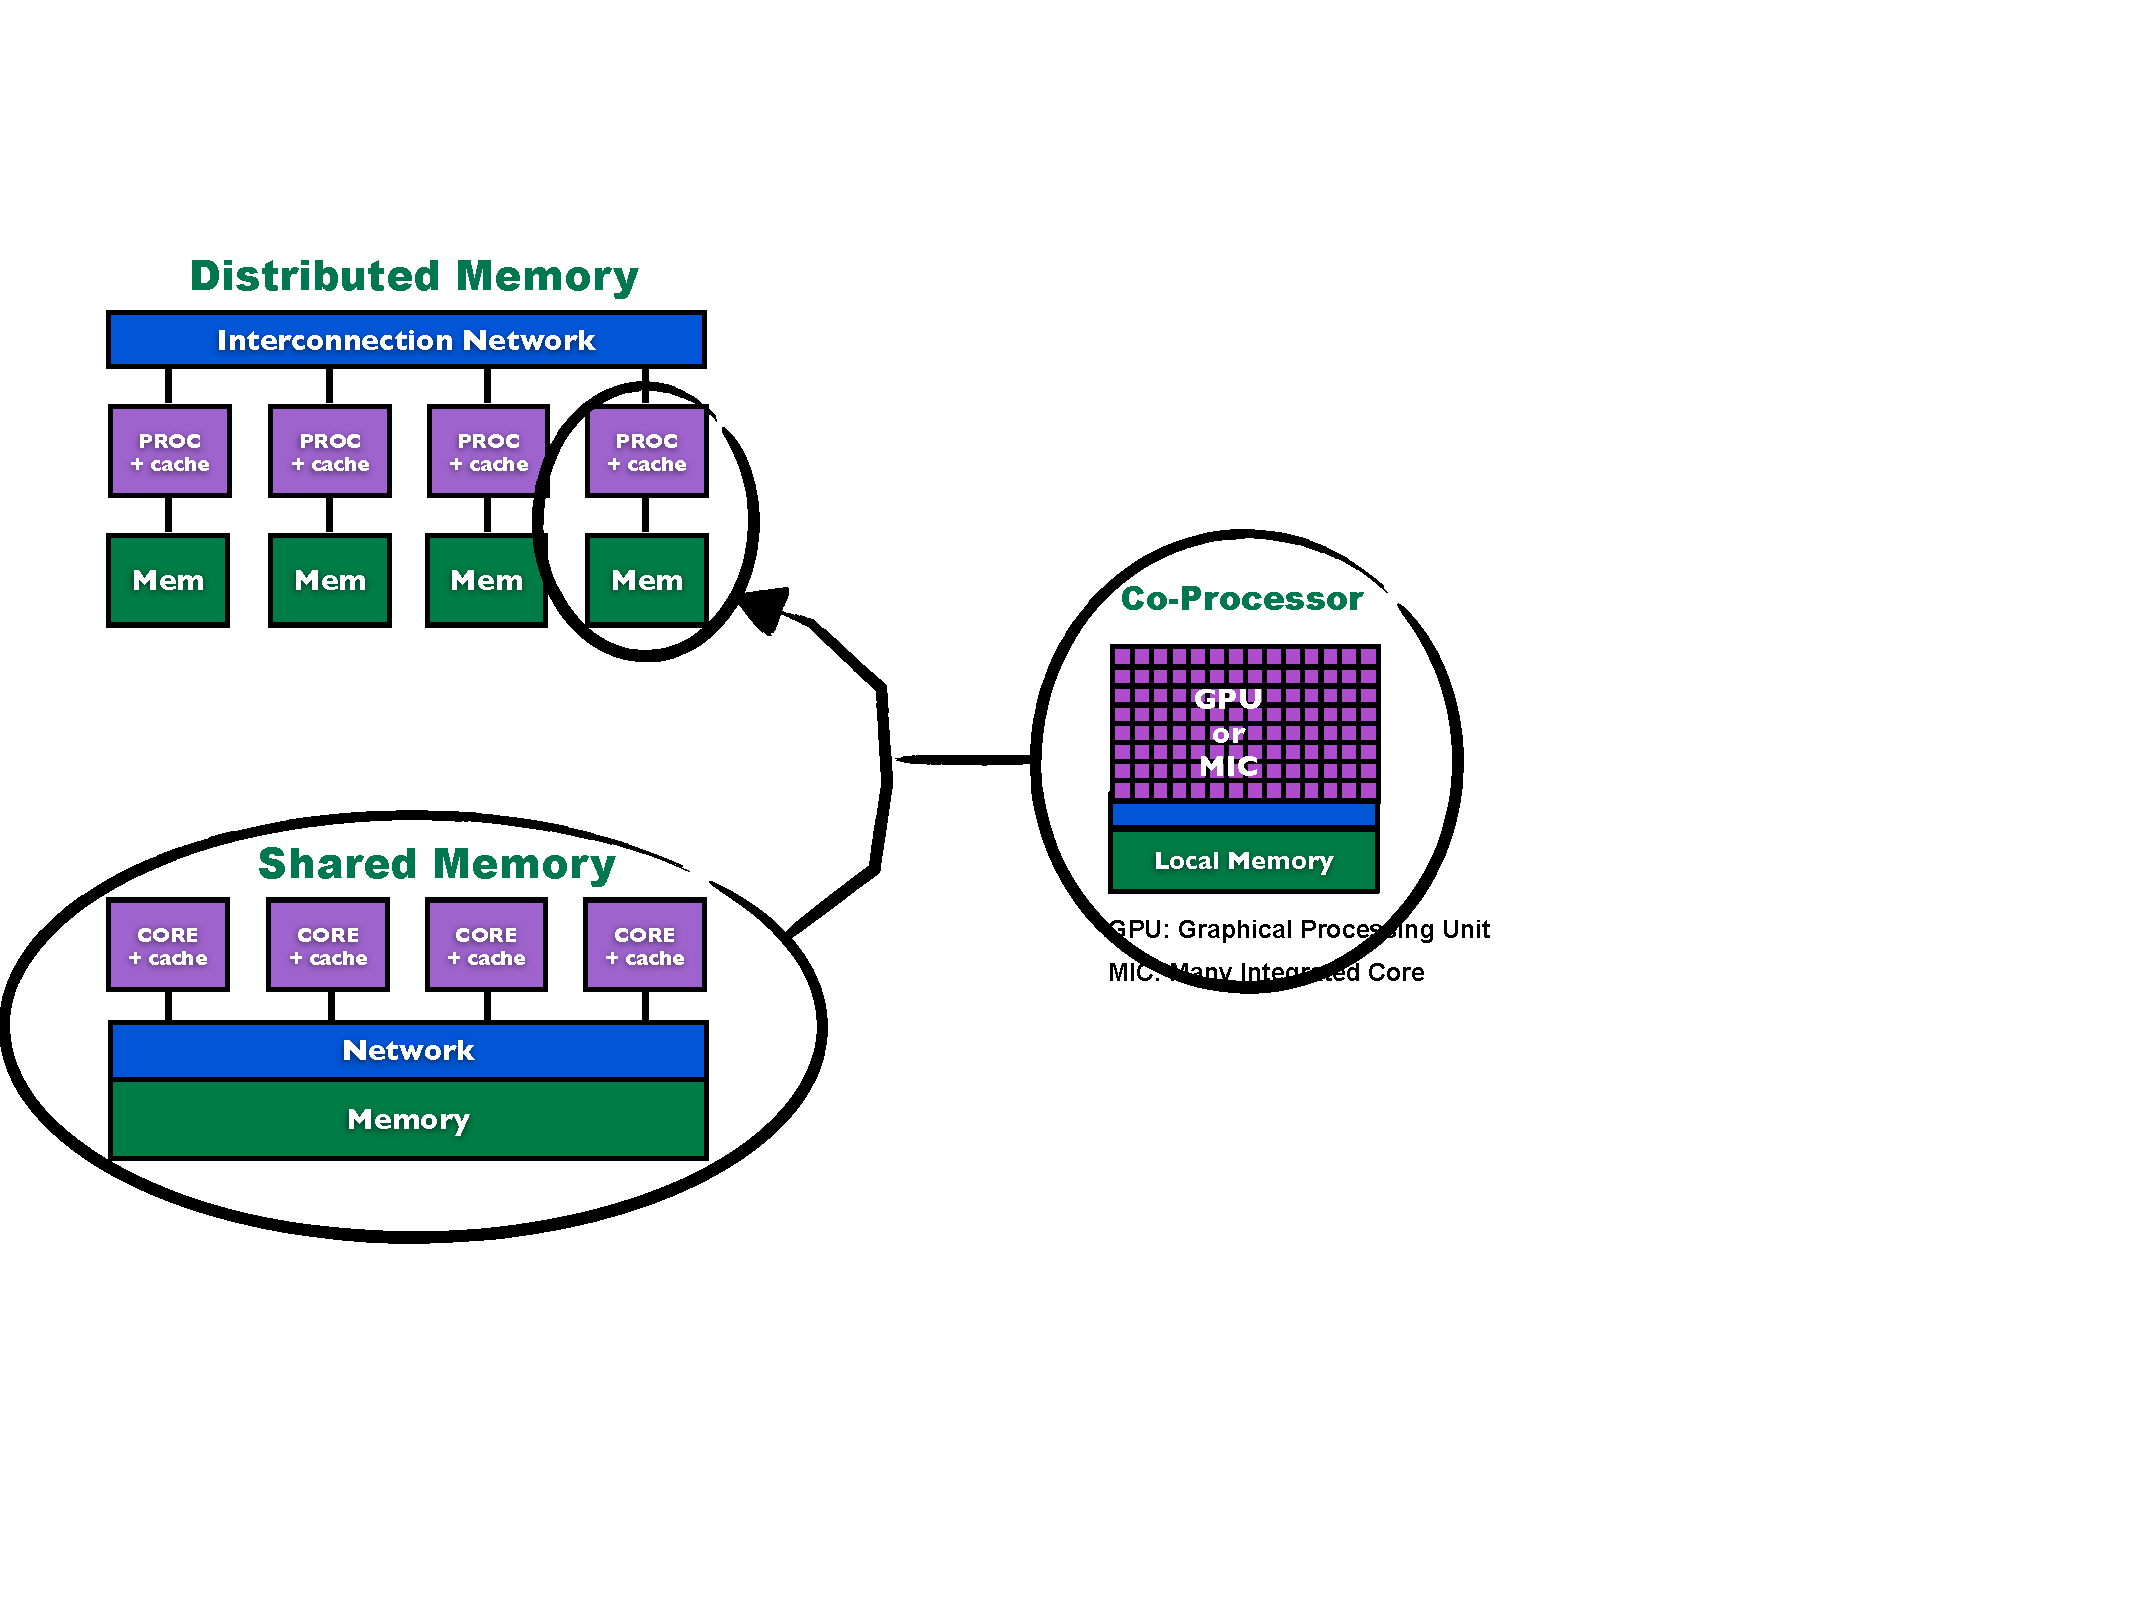
\includegraphics[width=0.95\textwidth]{pics/ParallelHardware4.pdf}
\end{block}
\end{frame}

\begin{frame}
\begin{block}{Knowing the Right Words}
    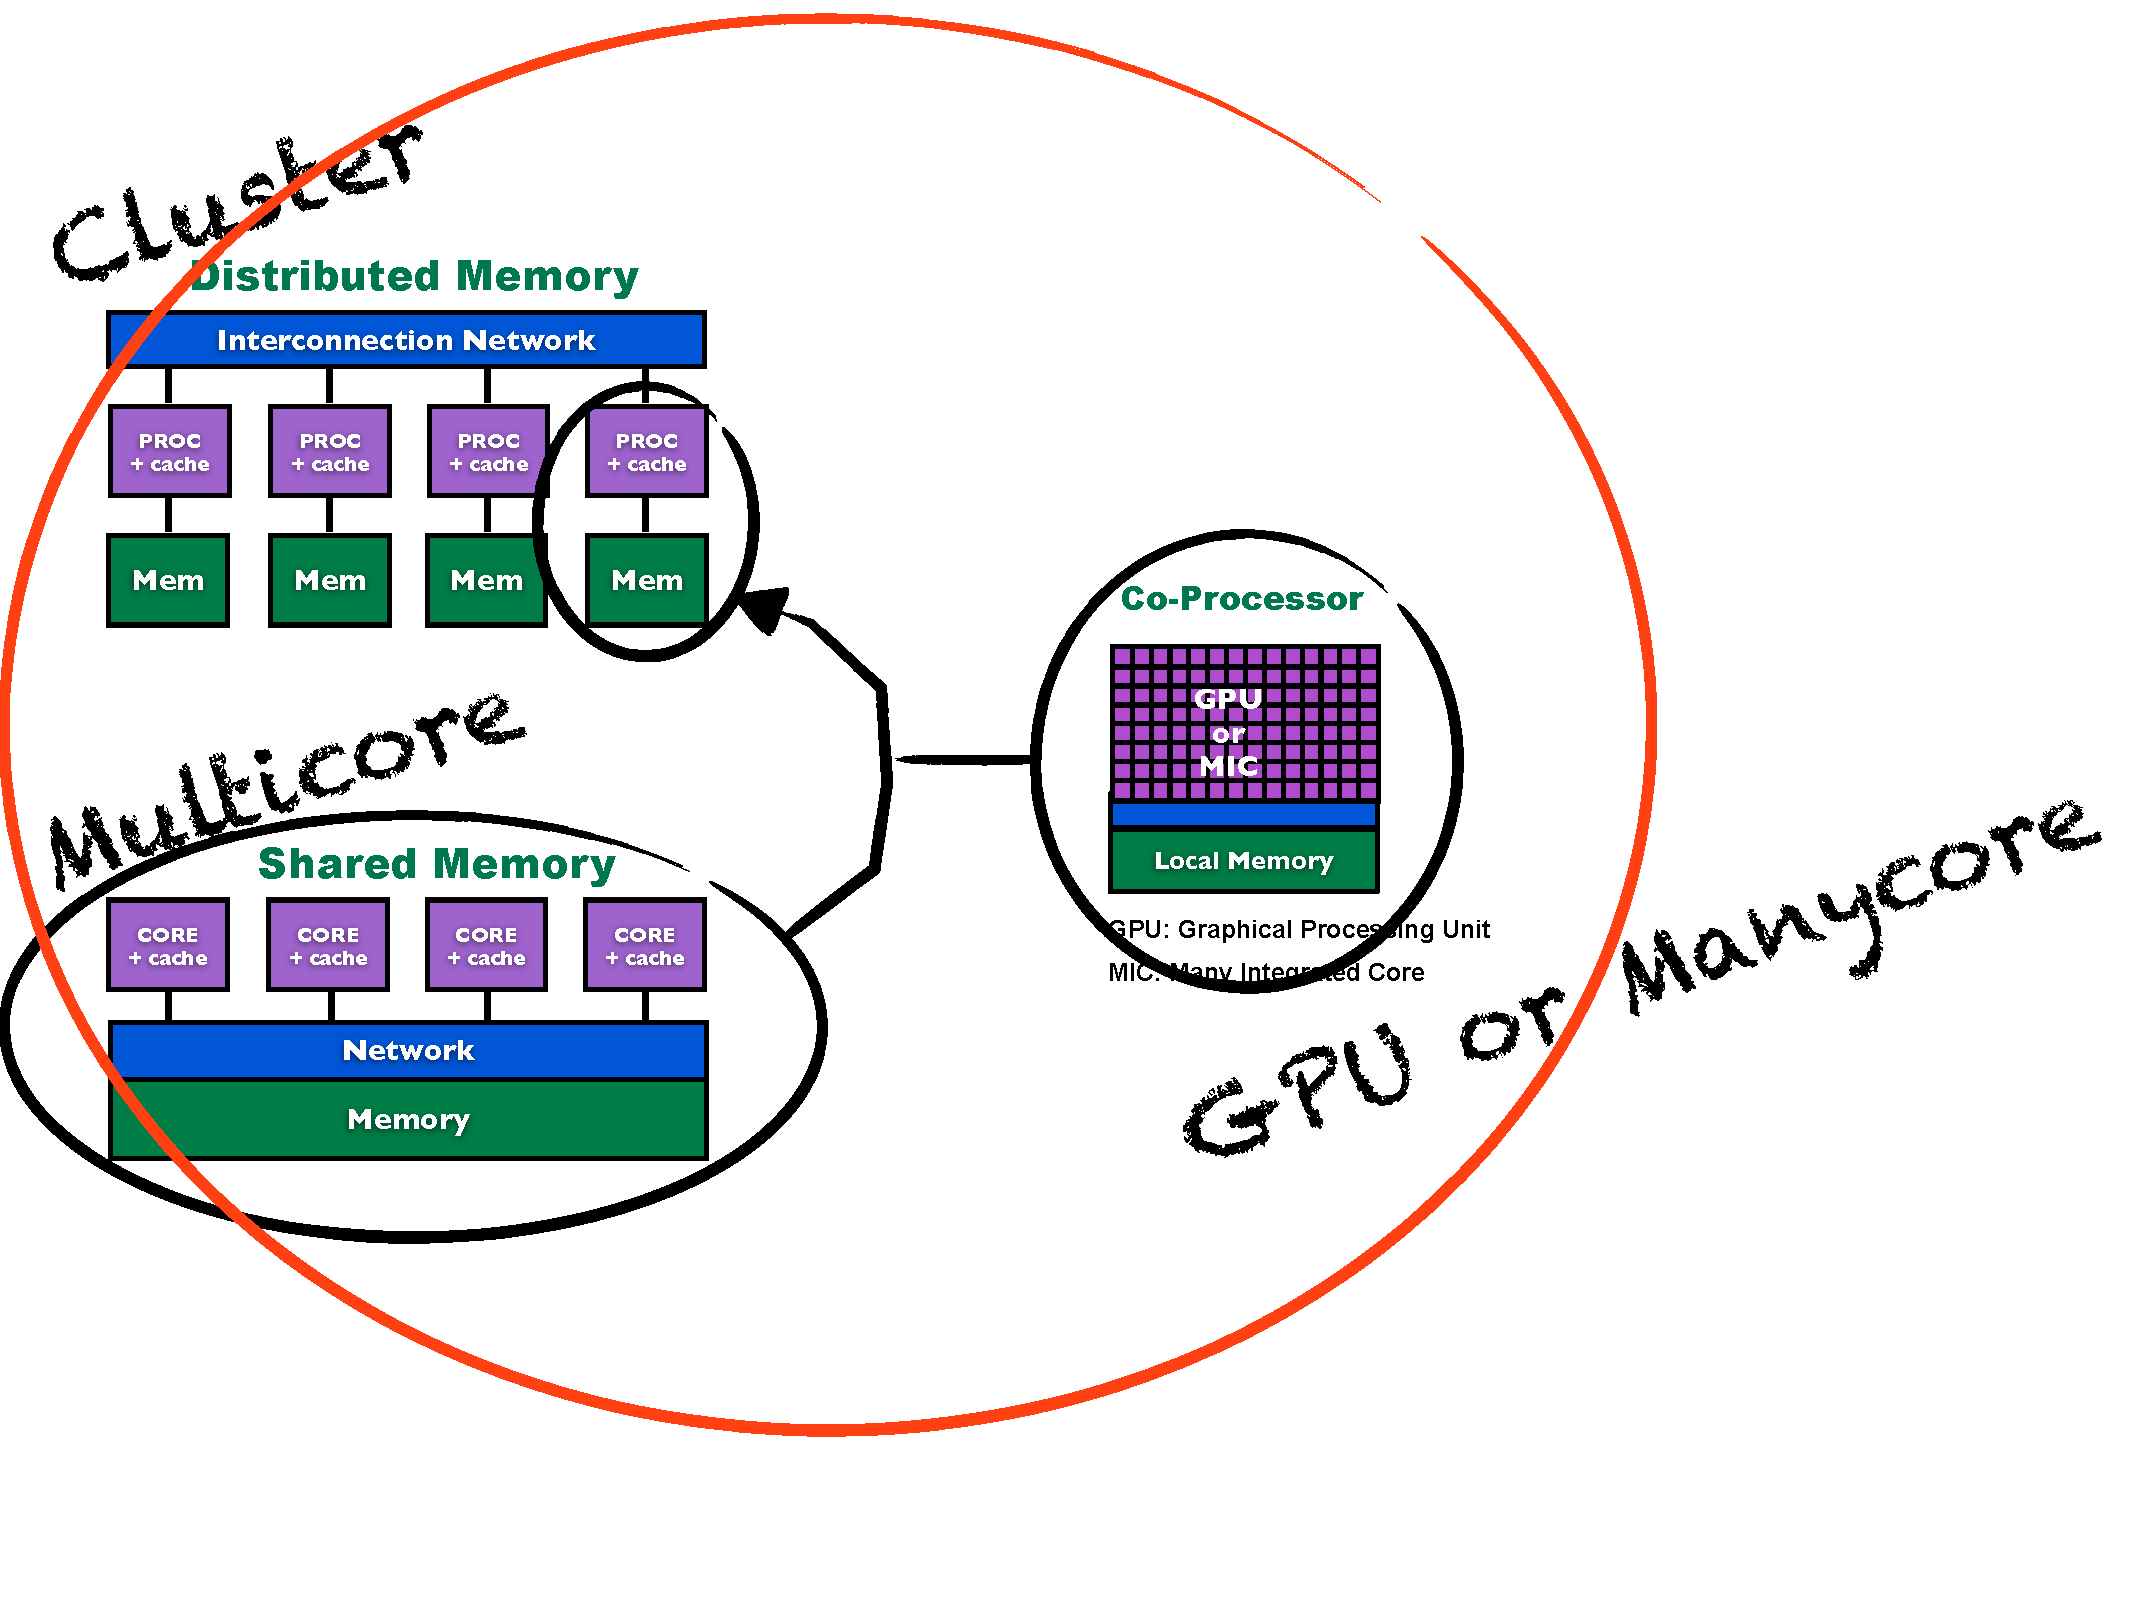
\includegraphics[width=0.95\textwidth]{pics/ParallelHardware5.pdf}
\end{block}
\end{frame}

\begin{frame}
\begin{block}{``Native'' Programming Models and Tools}
    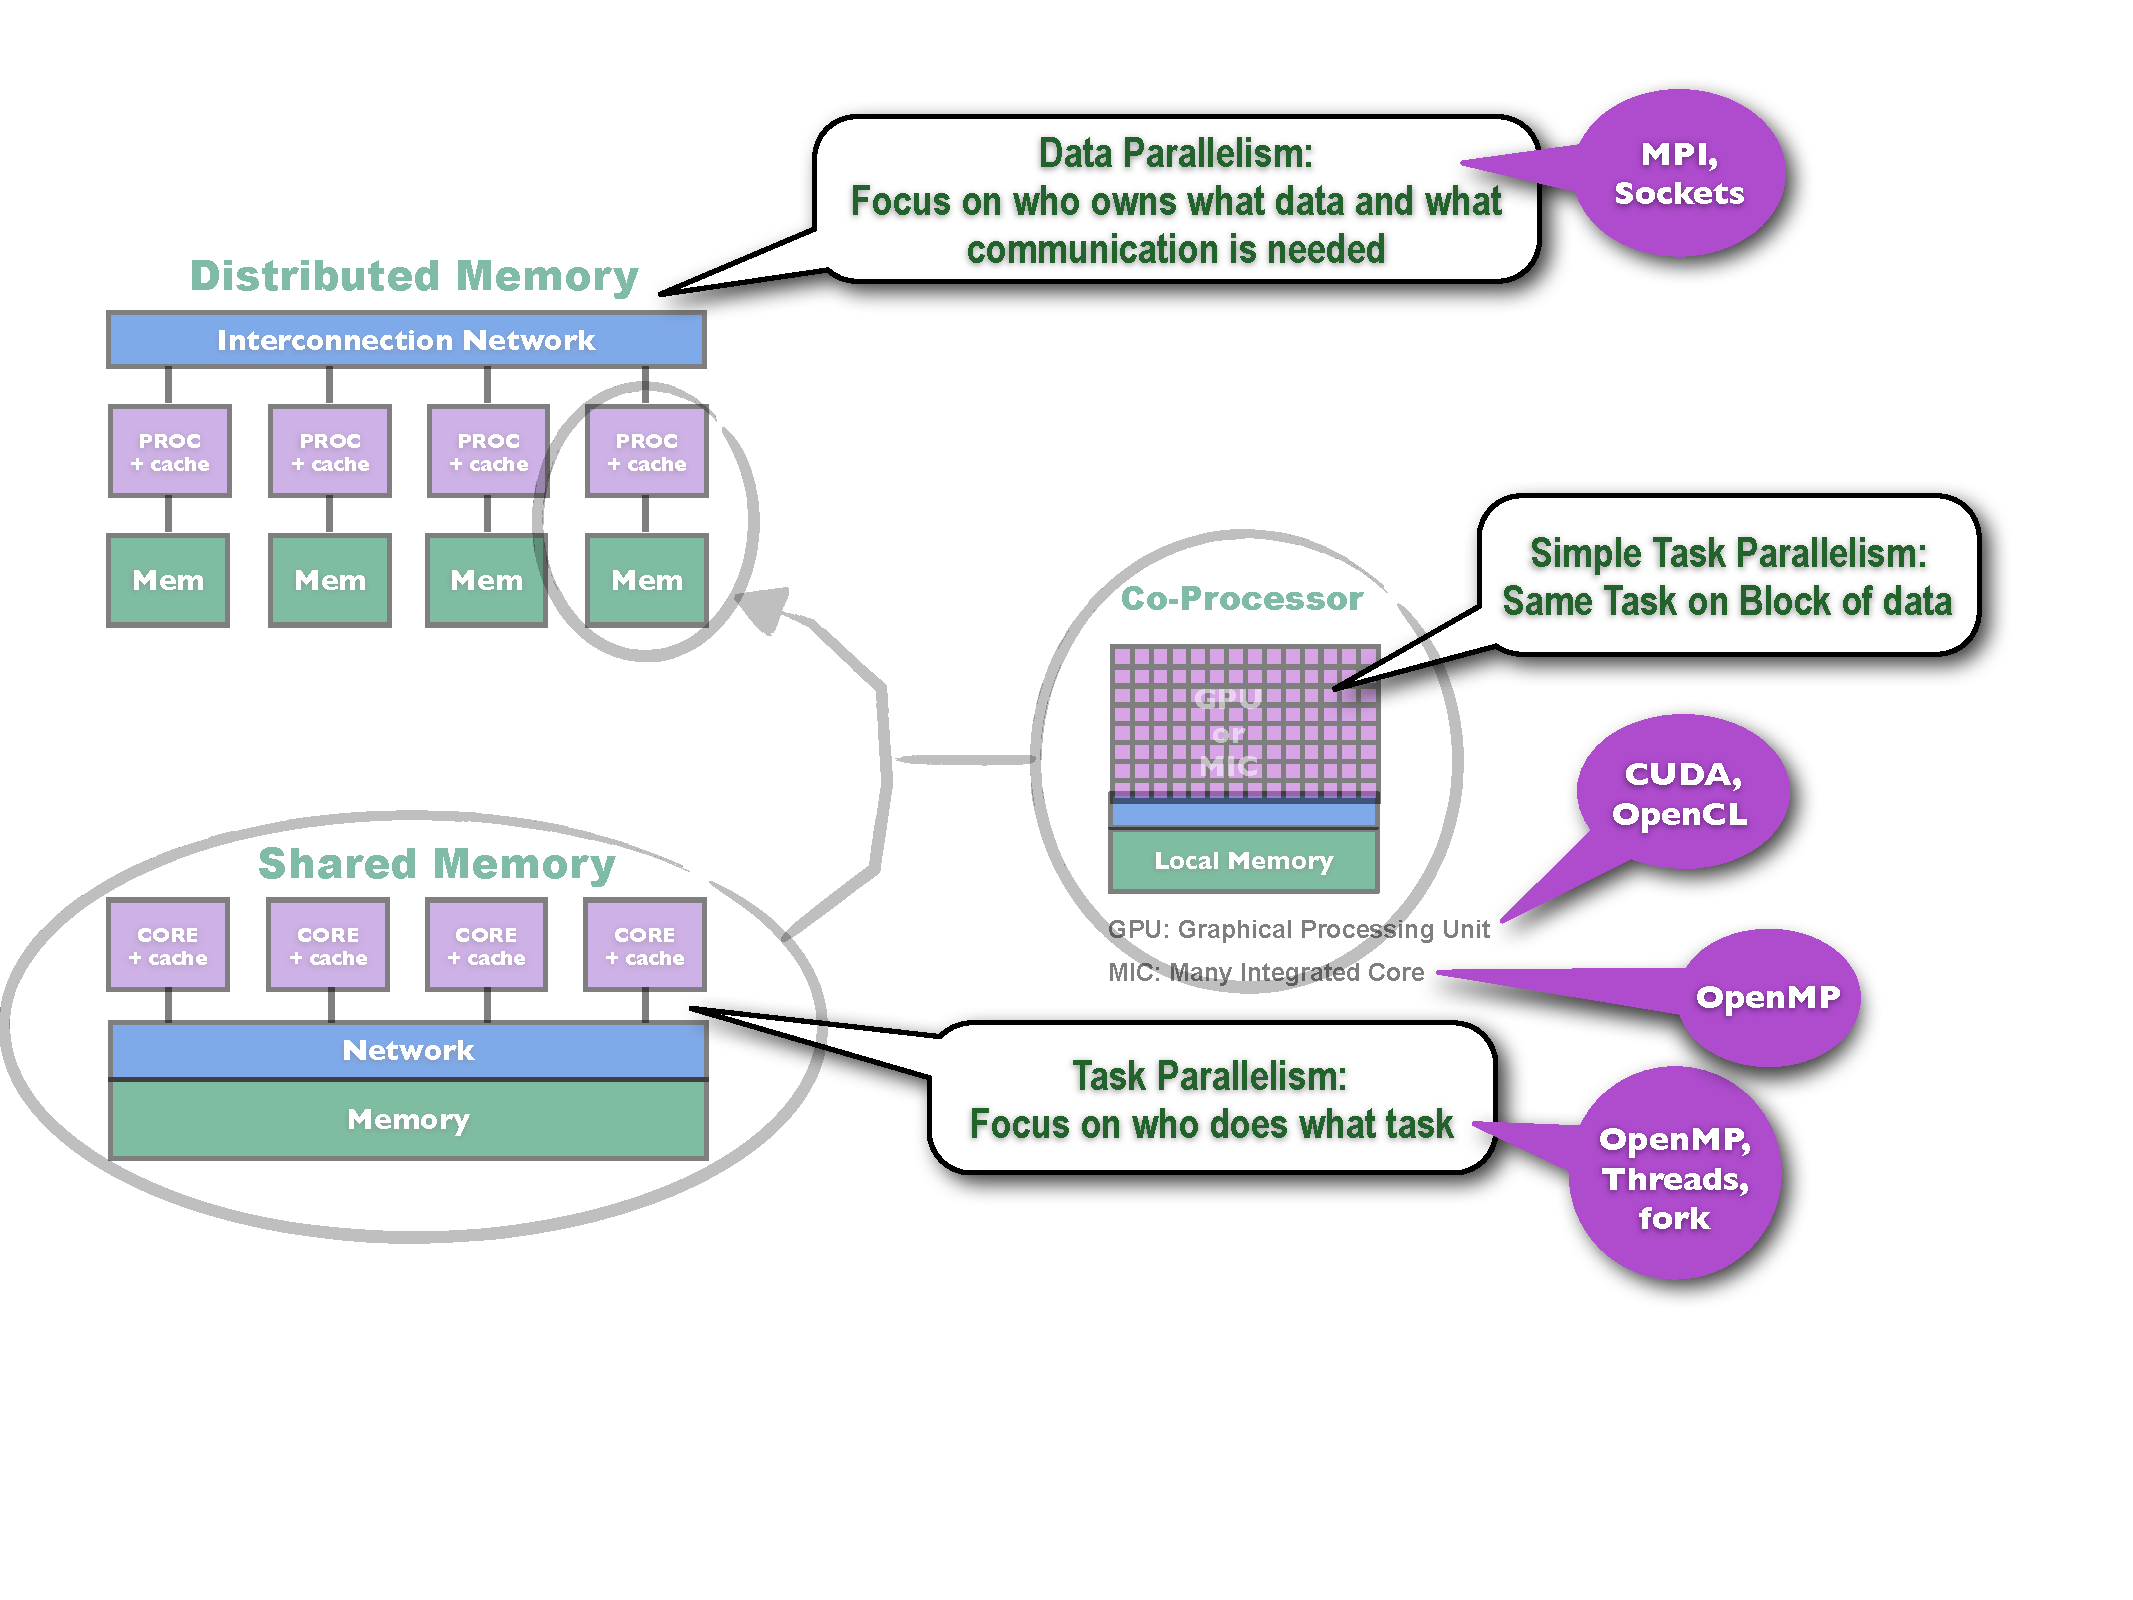
\includegraphics[width=0.95\textwidth]{pics/ParallelHardware6.pdf}
\end{block}
\end{frame}

\begin{frame}
\begin{block}{R Interfaces to Native Tools}
    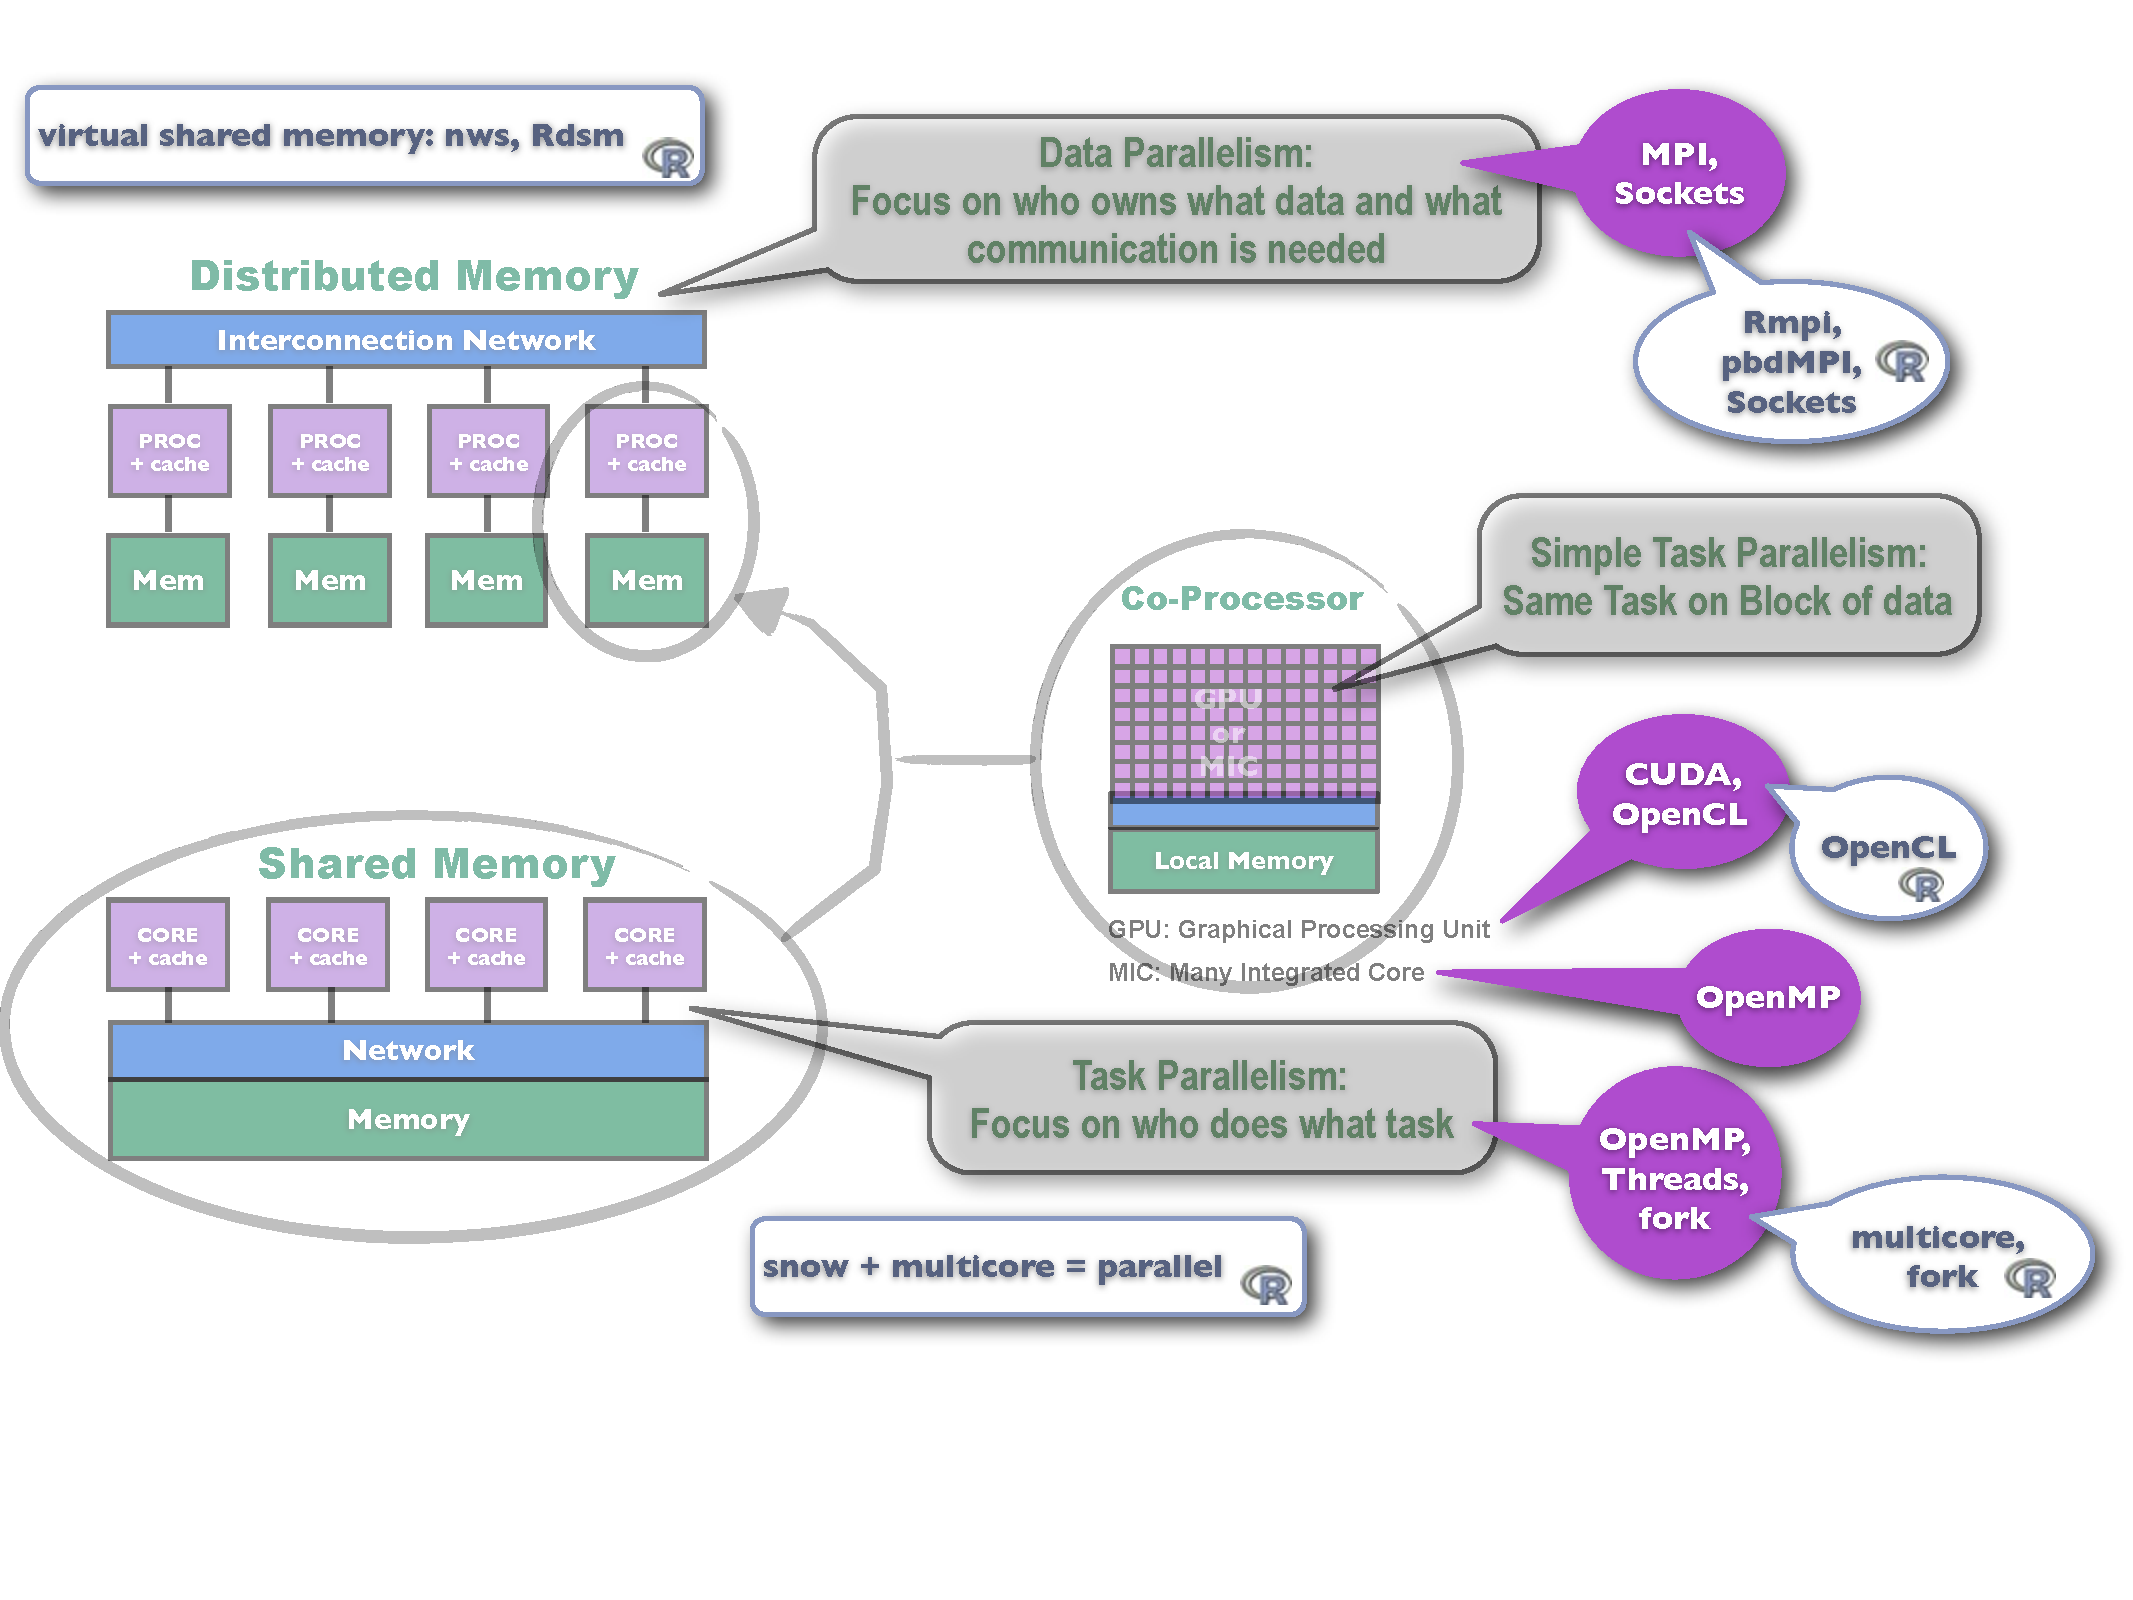
\includegraphics[width=0.95\textwidth]{pics/ParallelHardware7.pdf}
\end{block}
\end{frame}

\begin{frame}
\begin{block}{30+ Years of Parallel Computing Research}
    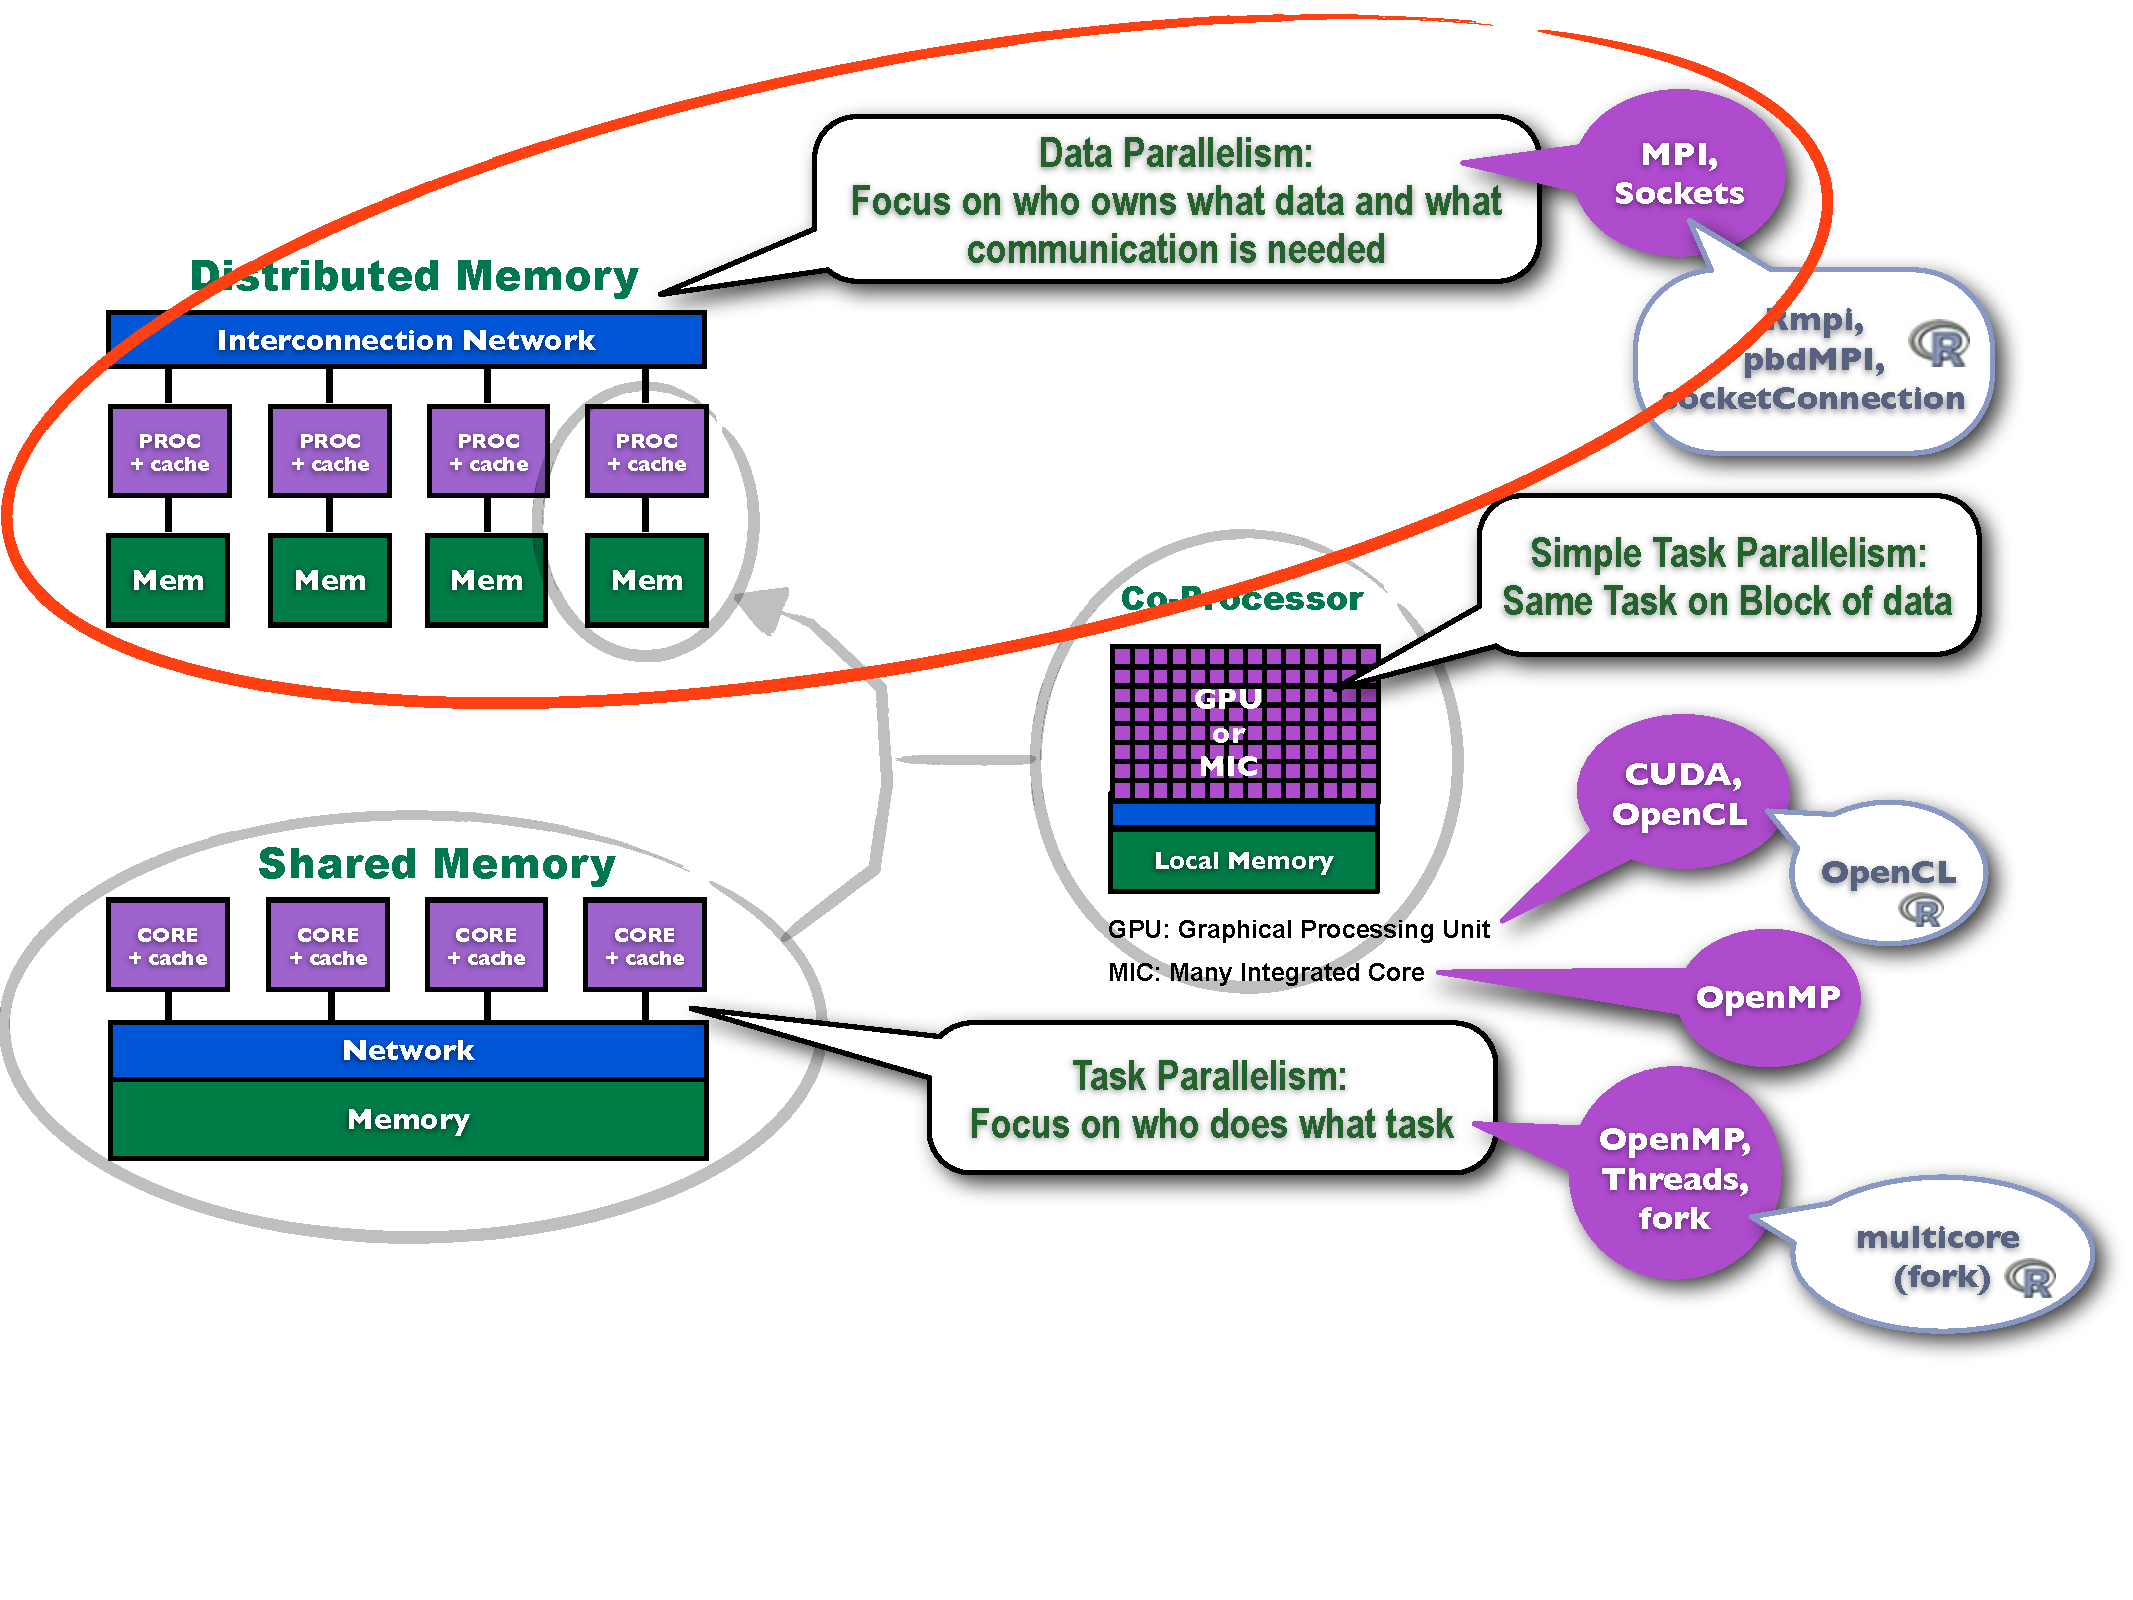
\includegraphics[width=0.95\textwidth]{pics/ParallelHardware8.pdf}
\end{block}
\end{frame}

\begin{frame}
\begin{block}{Last 10 years of Advances}
    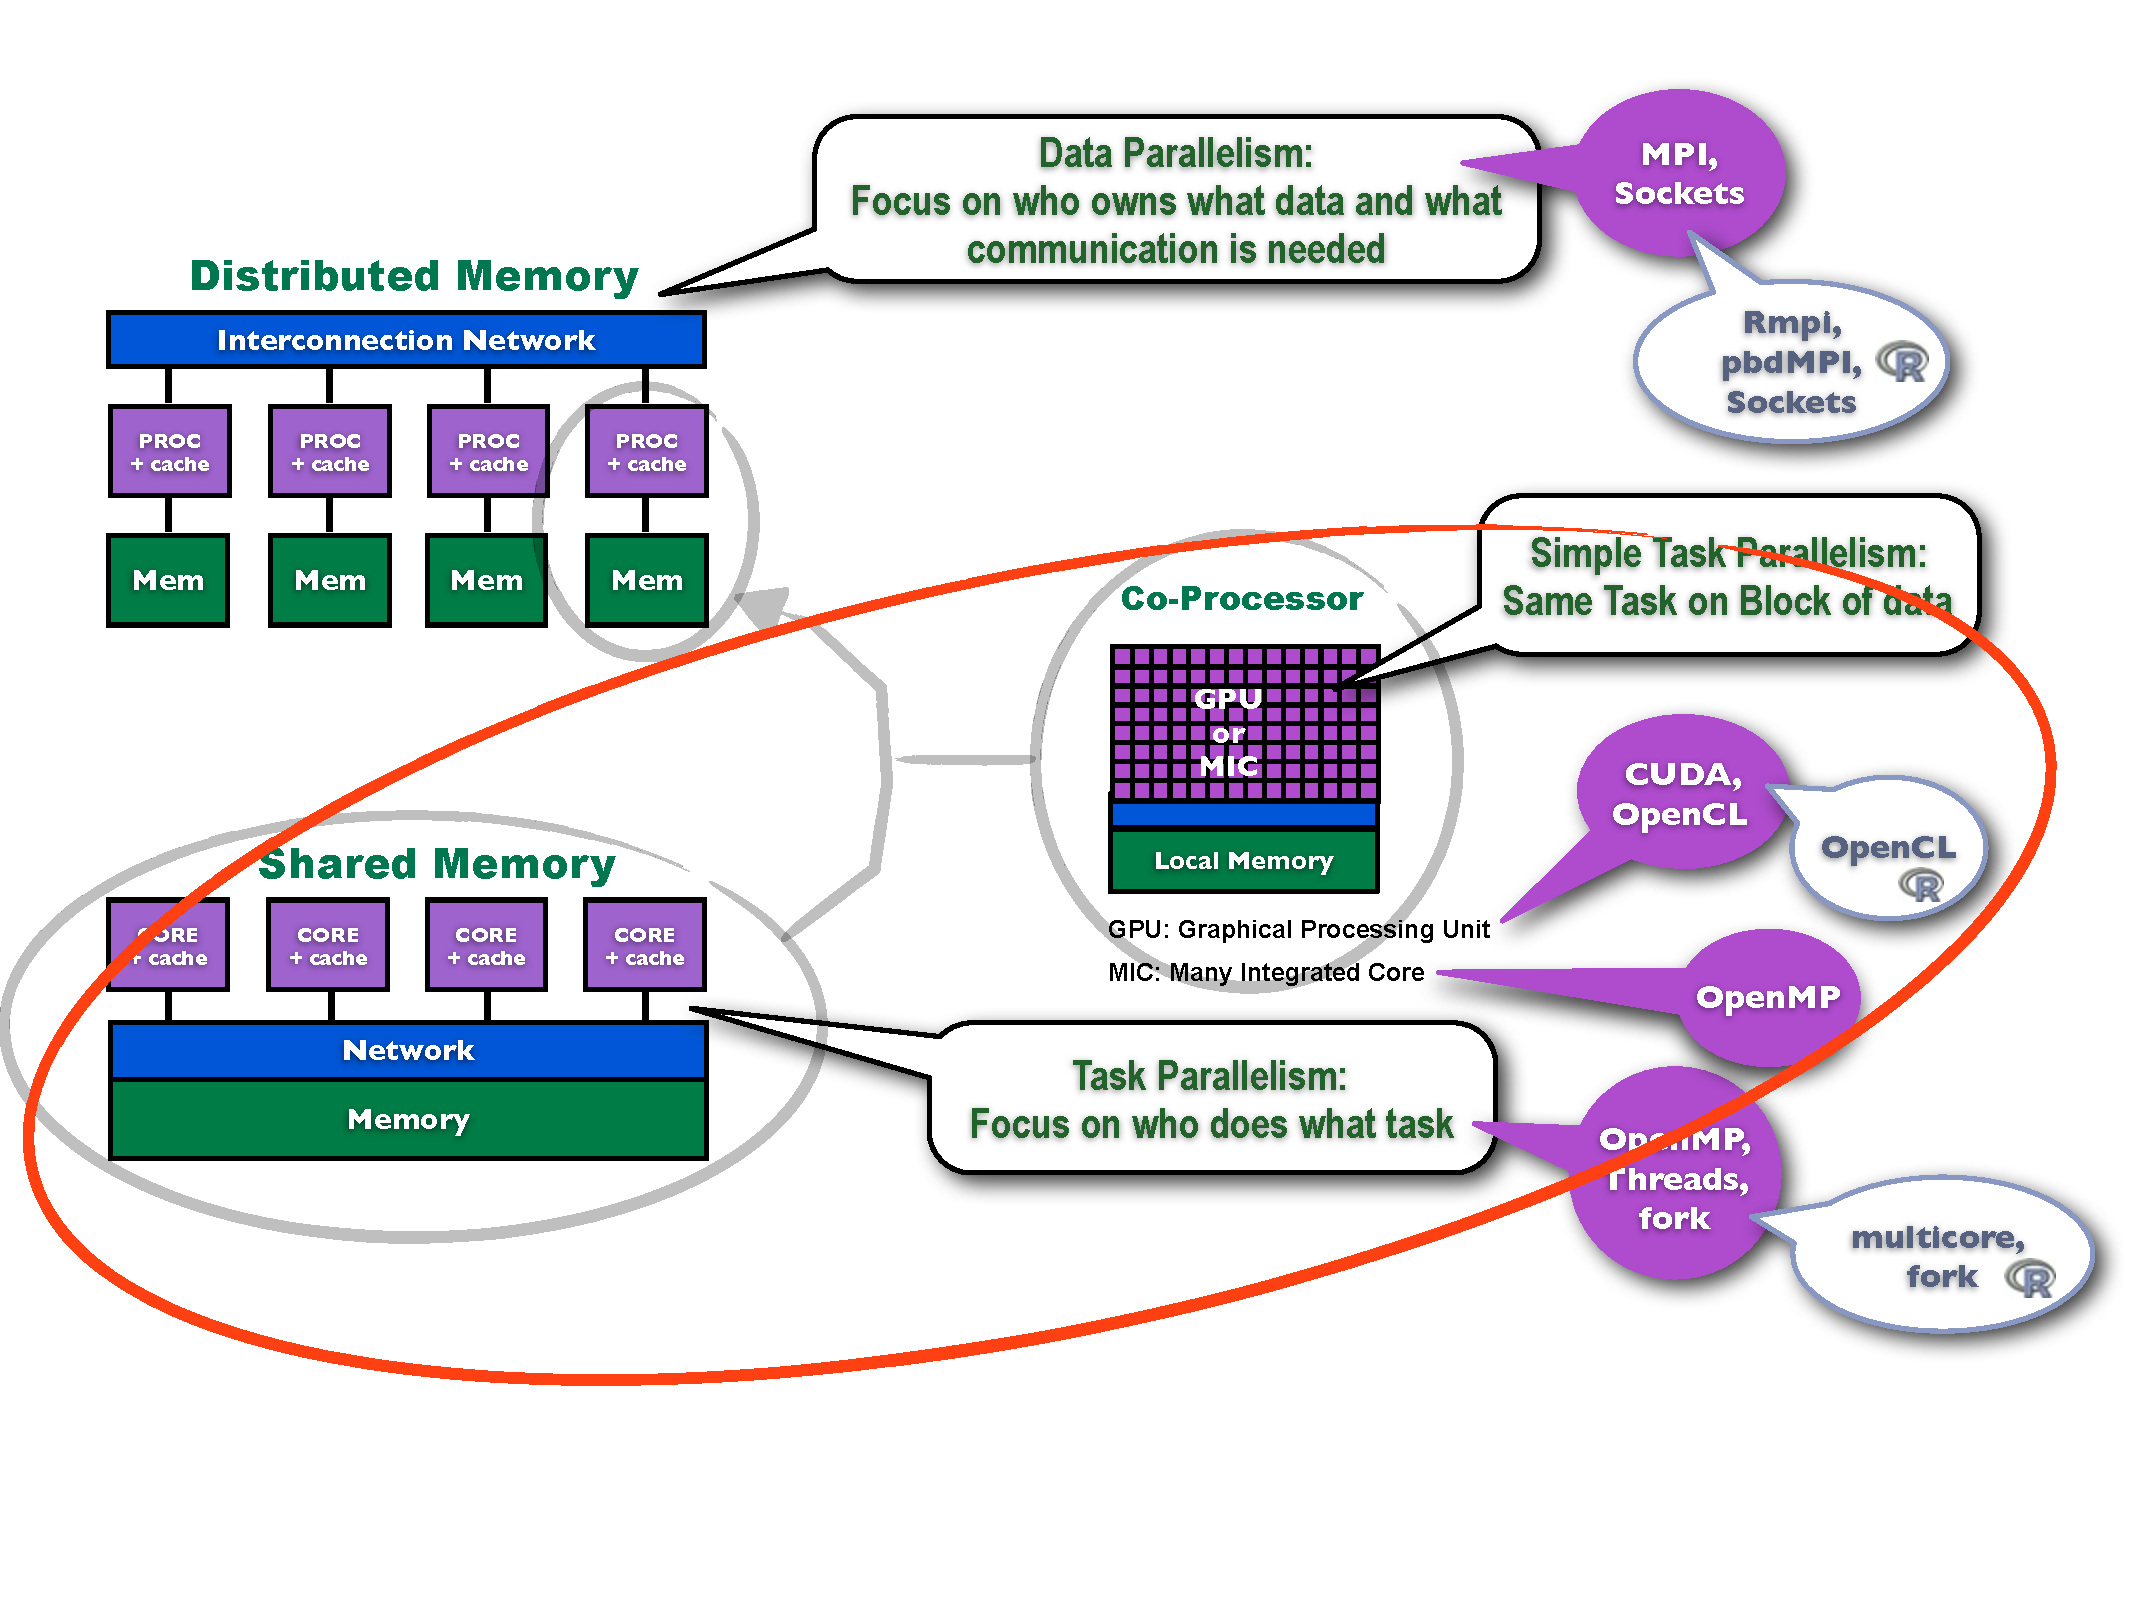
\includegraphics[width=0.95\textwidth]{pics/ParallelHardware9.pdf}
\end{block}
\end{frame}

\begin{frame}
\begin{block}{Putting It All Together Challenge}
    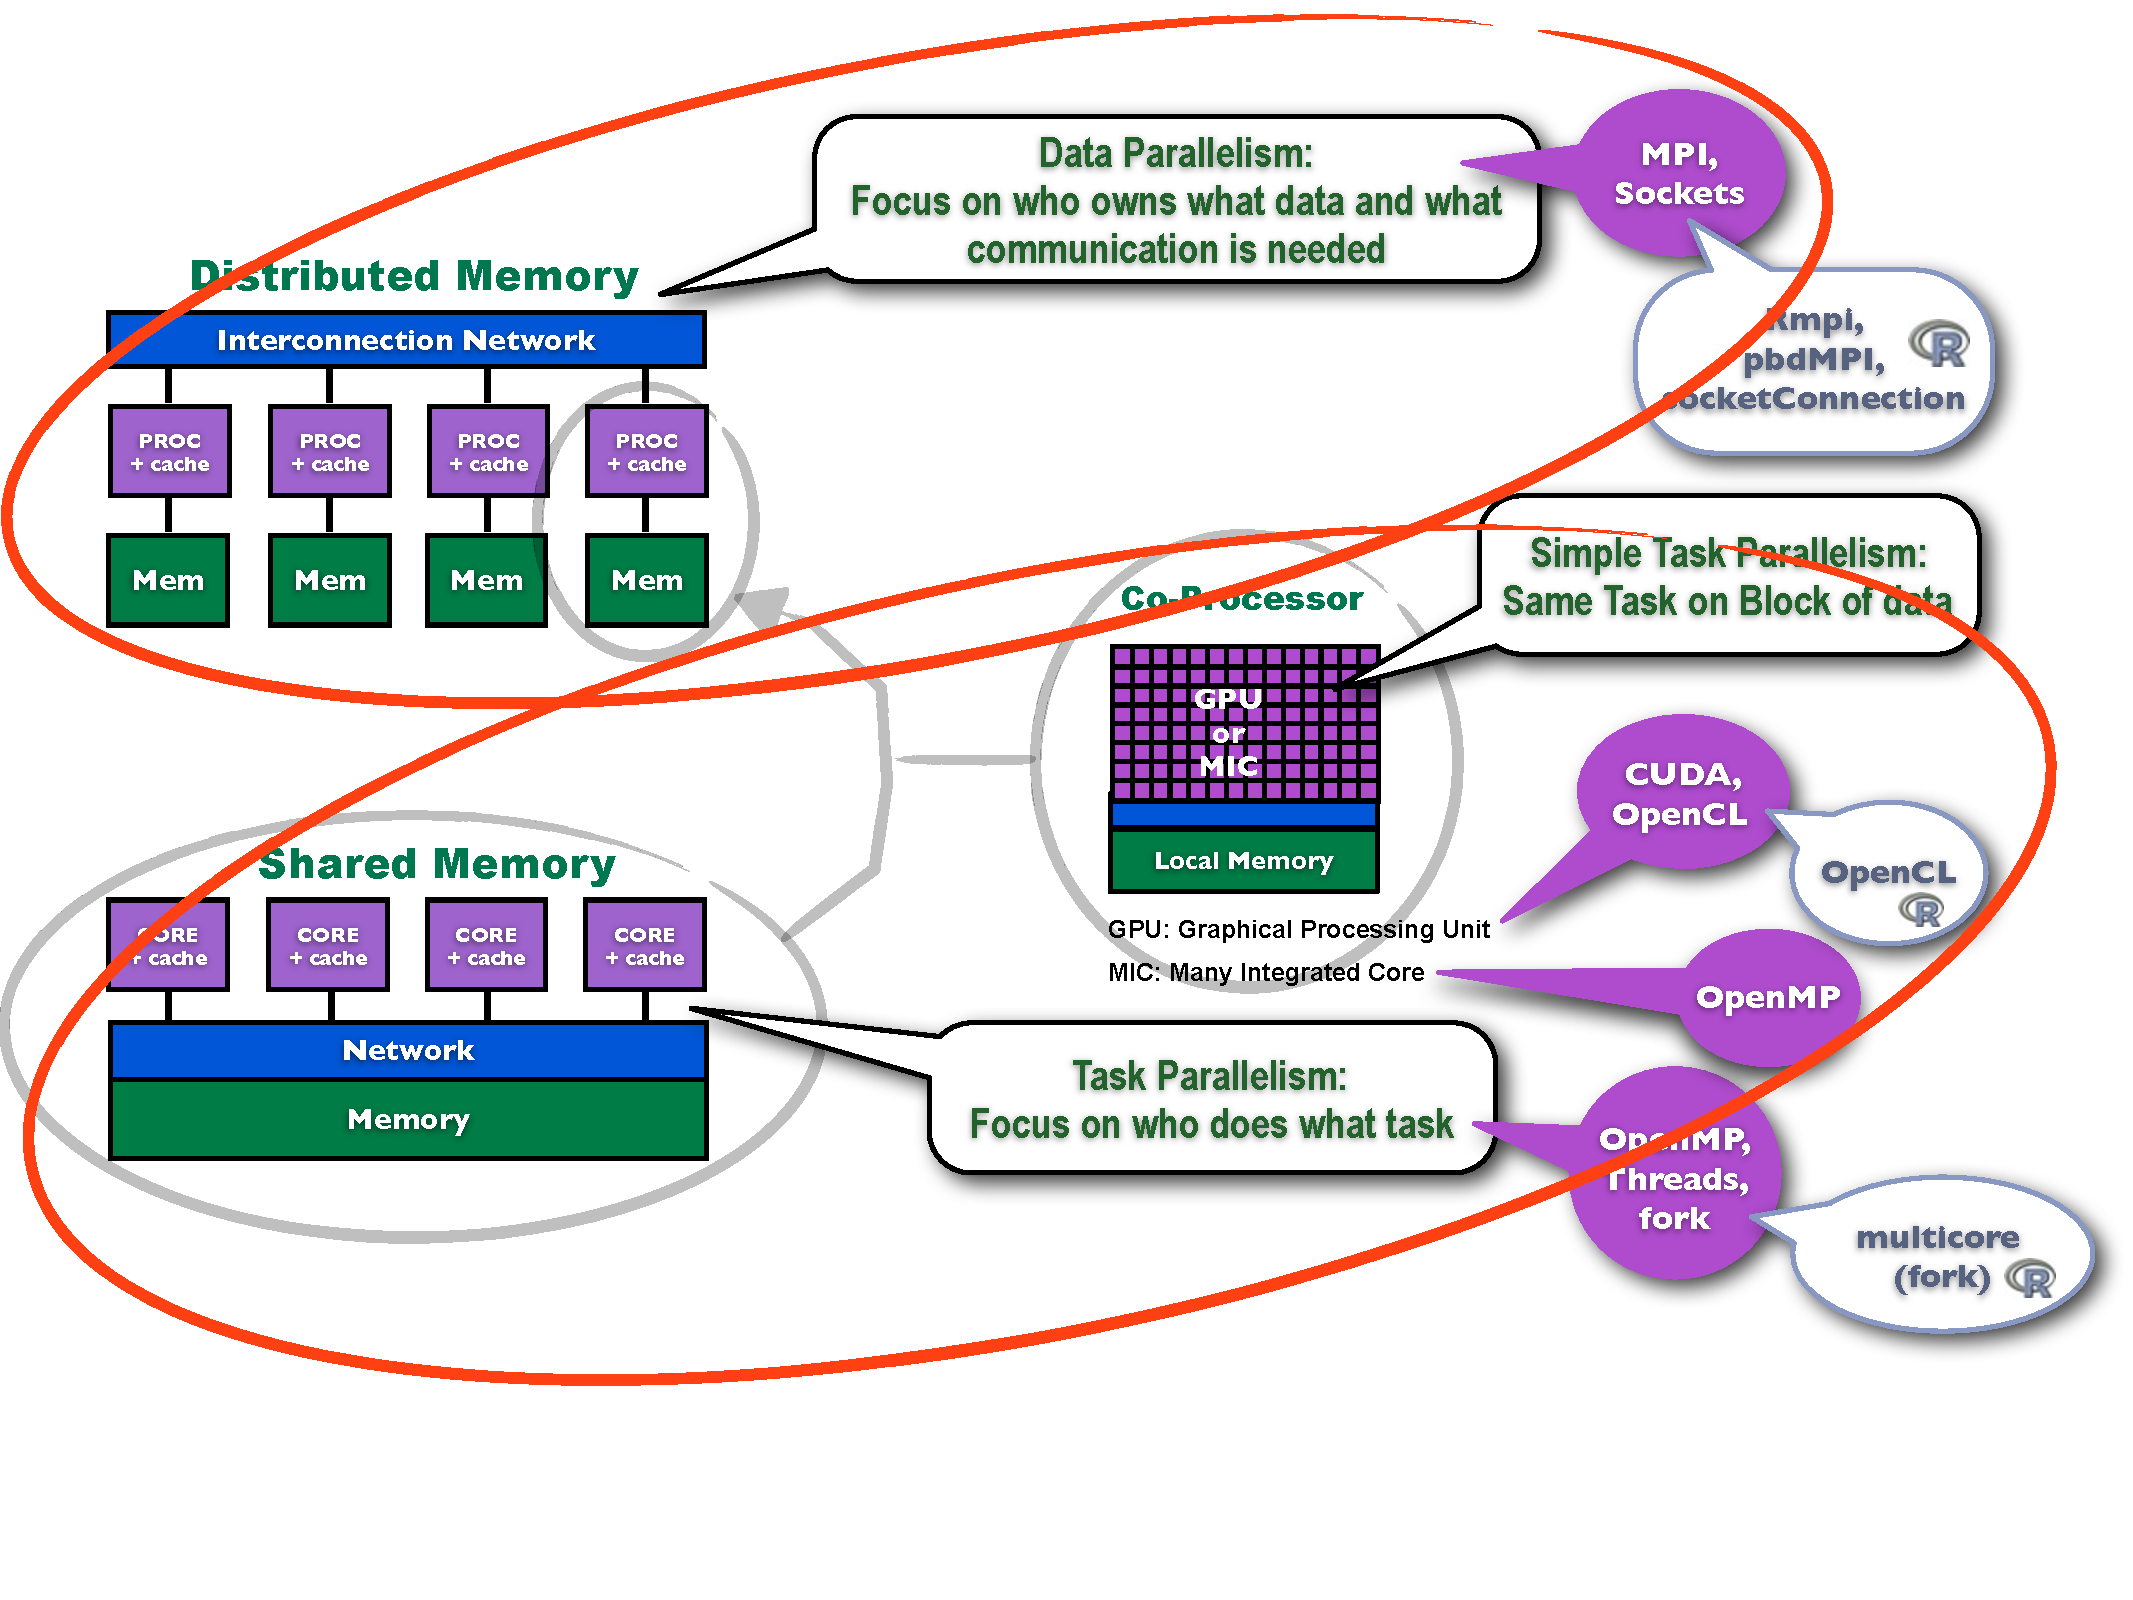
\includegraphics[width=0.95\textwidth]{pics/ParallelHardware10.pdf}
\end{block}
\end{frame}

\begin{frame}
\begin{block}{pbdR Focus on Data Parallelism}
    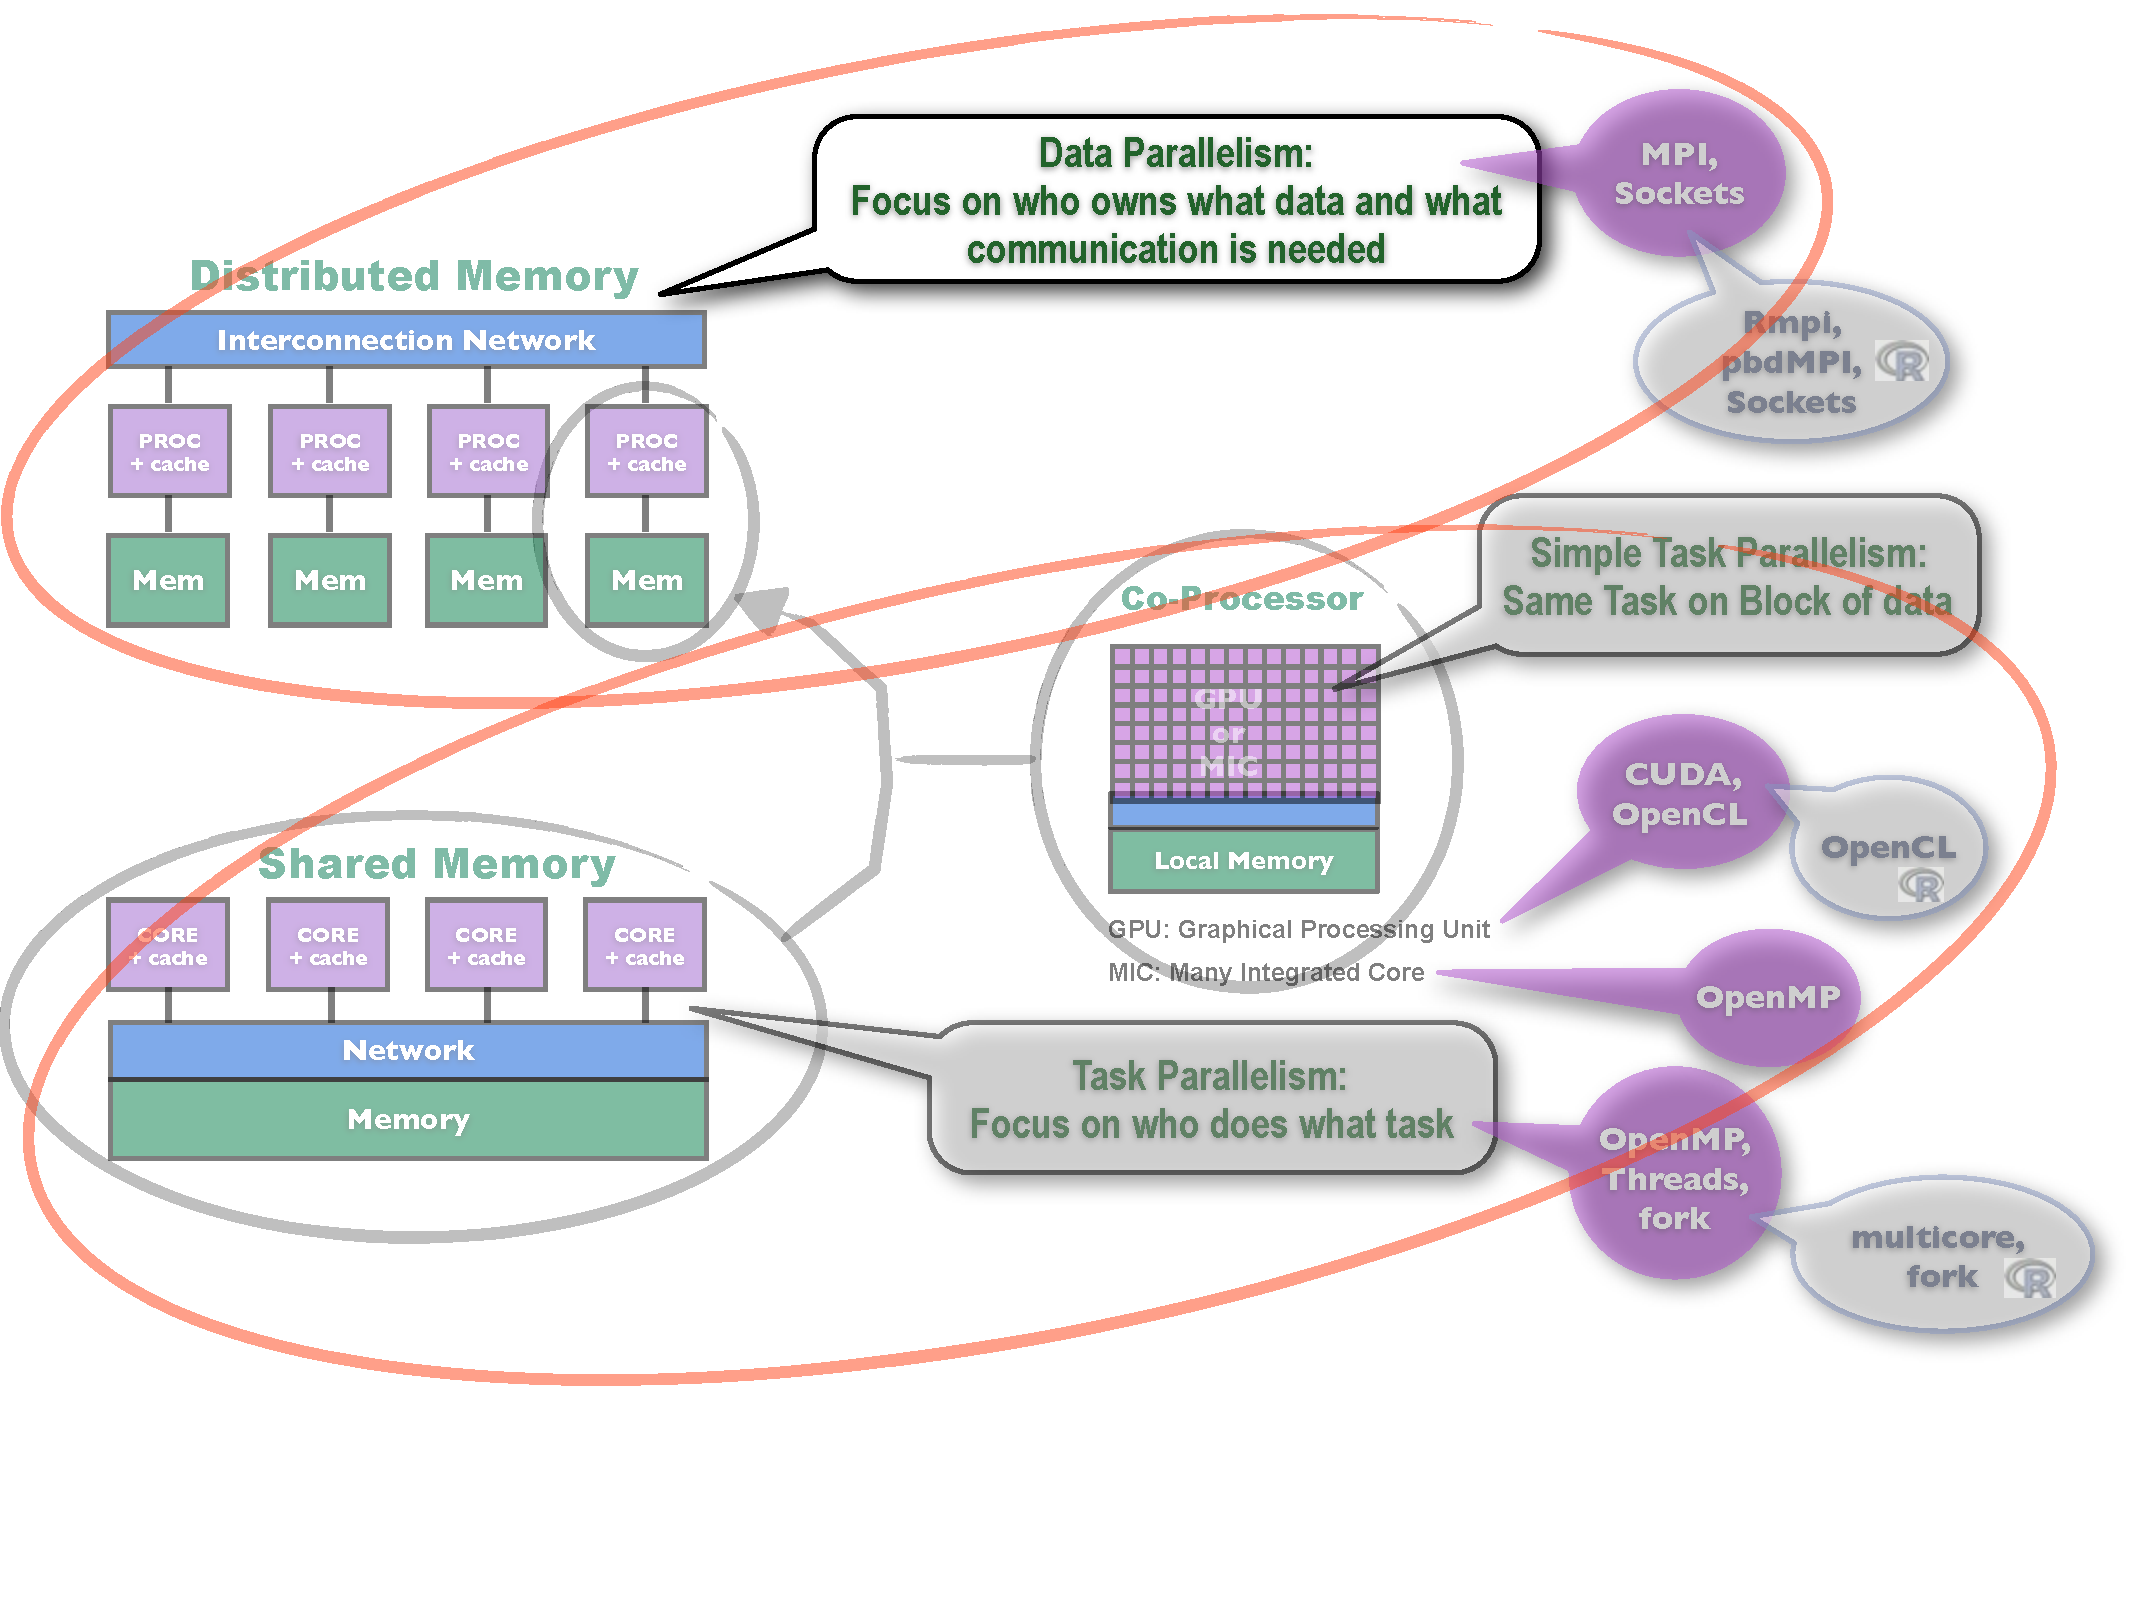
\includegraphics[width=0.95\textwidth]{pics/ParallelHardware11.pdf}
\end{block}
\end{frame}

\setcounter{framenumber}{0}

\subsection{A Concise Introduction to Parallelism}

\begin{frame}
  \begin{block}{What is Parallelism?}\pause
  Broadly, \emph{doing more than one thing at a time}.\\[.2cm]
  
  The simultaneous use of multiple compute resources to solve a computational problem: 
  \end{block}
\end{frame}

\begin{frame}
  \begin{block}{Parallelism}\pause
    \begin{center}
    \begin{minipage}{.46\textwidth}
    \begin{block}{\centering Serial Programming}
      \begin{center}
      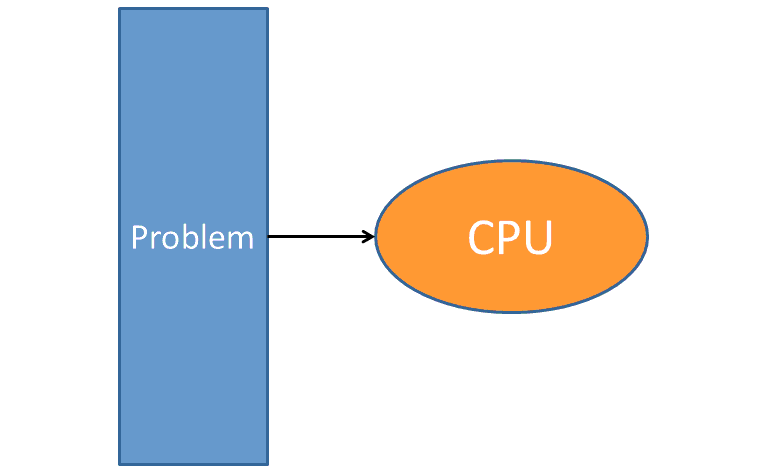
\includegraphics[width=.975\textwidth]{pics/parallelism1}
      \end{center}
      \end{block}
    \end{minipage}
    \hspace{.15cm}
    \begin{minipage}{.46\textwidth}
    \begin{block}{\centering Parallel Programming}
      \begin{center}
      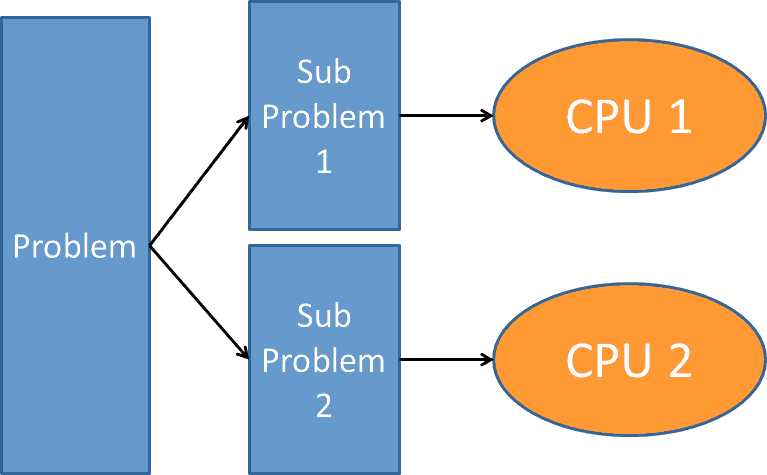
\includegraphics[width=.975\textwidth]{pics/parallelism2}
      \end{center}
      \end{block}
    \end{minipage}
    \end{center}
  \end{block}
\end{frame}

\begin{frame}
  \begin{block}{Parallelism}\pause
    \begin{center}
    \begin{minipage}{.46\textwidth}
    \begin{block}{Serial Programming}
      \begin{center}
      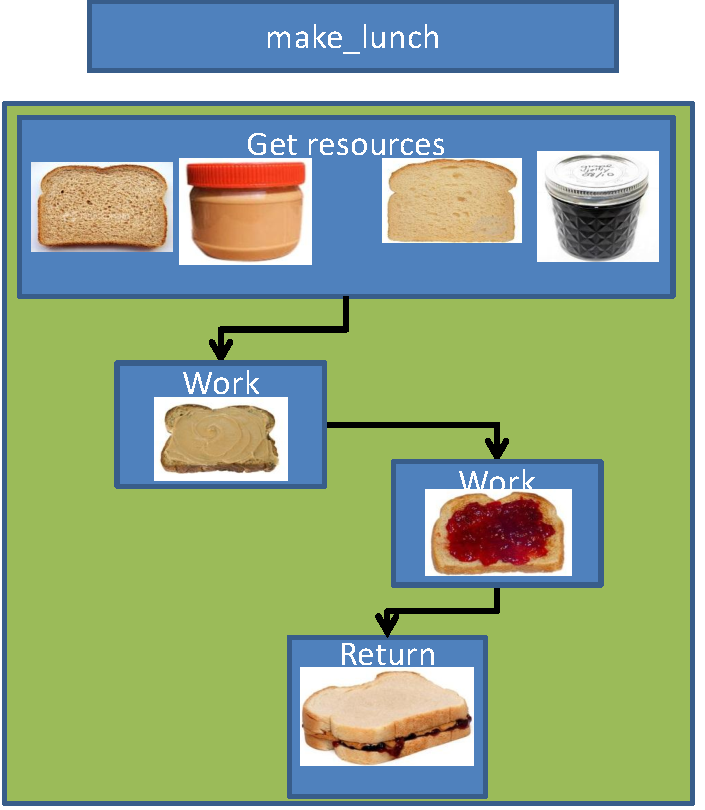
\includegraphics[width=.975\textwidth]{pics/analogy_serial}
      \end{center}
      \end{block}
    \end{minipage}
    \hspace{.15cm}
    \begin{minipage}{.46\textwidth}
    \begin{block}{Parallel Programming}
      \begin{center}
      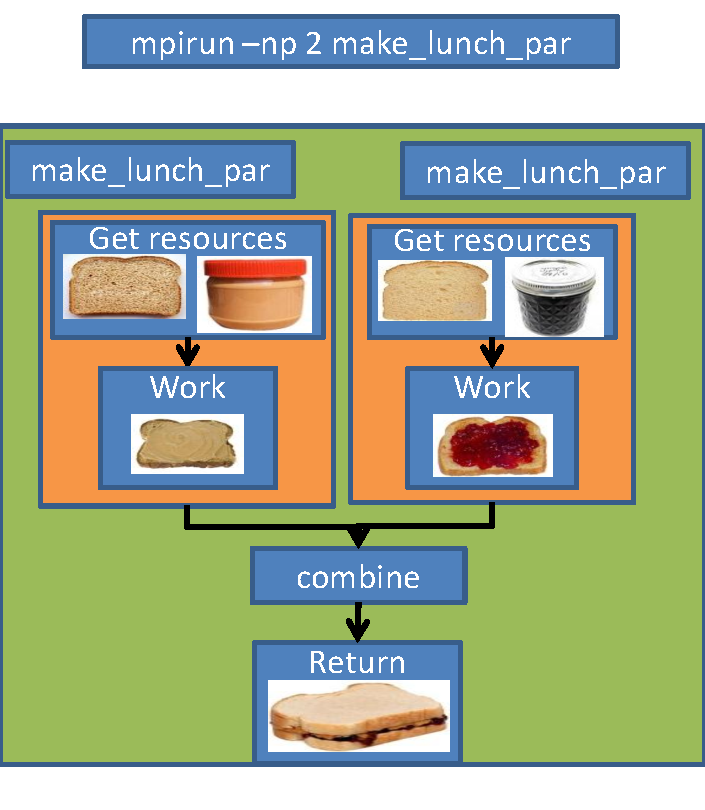
\includegraphics[height=5.45cm,width=.975\textwidth]{pics/analogy_parallel}
      \end{center}
      \end{block}
    \end{minipage}
    \end{center}
  \end{block}
\end{frame}

% \begin{frame}
%   \begin{block}{What is Parallelism?}\pause
%   Broadly, \emph{doing more than one thing at a time}.\\
%     \begin{itemize}[<+-|alert@+>]
%    \item \emph{Task Parallelism}:  Many small tasks.\\
%    \emph{e.g.} Make one sandwich for each person on earth.
%    \item \emph{Data Parallelism}:  One really big task.\\
%    \emph{e.g.}  Make one sandwich so large that every person on earth could eat from it.\\
%   \end{itemize}
%   \end{block}
% \end{frame}

\begin{frame}
  \begin{block}{Kinds of Parallelism}\pause
    \begin{itemize}[<+-|alert@+>]
      \item \emph{Data Parallelism}:  Data is distributed
      \item \emph{Task Parallelism}:  Tasks are distributed
  \end{itemize}
  \end{block}
\end{frame}


\begin{frame}
  \begin{block}{pbdR Paradigms:  Data Parallelism}
  With data parallelism:
  \begin{itemize}[<+-|alert@+>]
   \item No one processor/node owns all the data.
   \item Processors own local pieces of a (conceptually) global object
  \end{itemize}
  \end{block}
\end{frame}


\begin{frame}
  \begin{block}{Data vs Task Parallelism}\pause
    \begin{center}
    \begin{minipage}{.46\textwidth}
    \begin{block}{\centering Data Parallelism}
      \begin{center}
      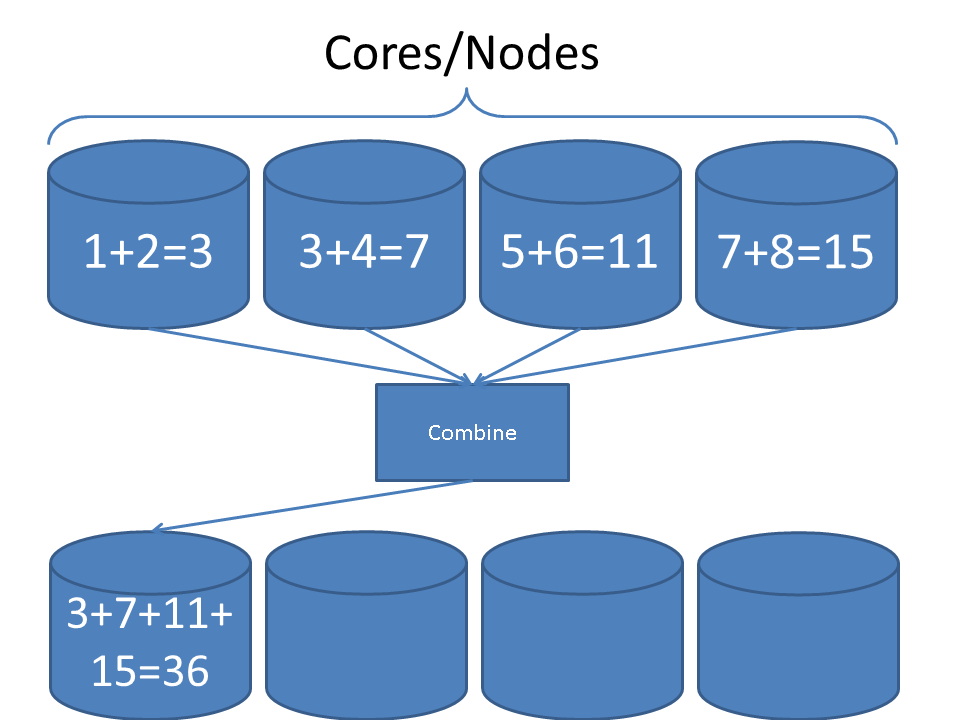
\includegraphics[width=.975\textwidth]{pics/parallelism_data}
      \end{center}
      \end{block}
    \end{minipage}
    \hspace{.15cm}
    \begin{minipage}{.46\textwidth}
    \begin{block}{\centering Task Parallelism}
      \begin{center}
      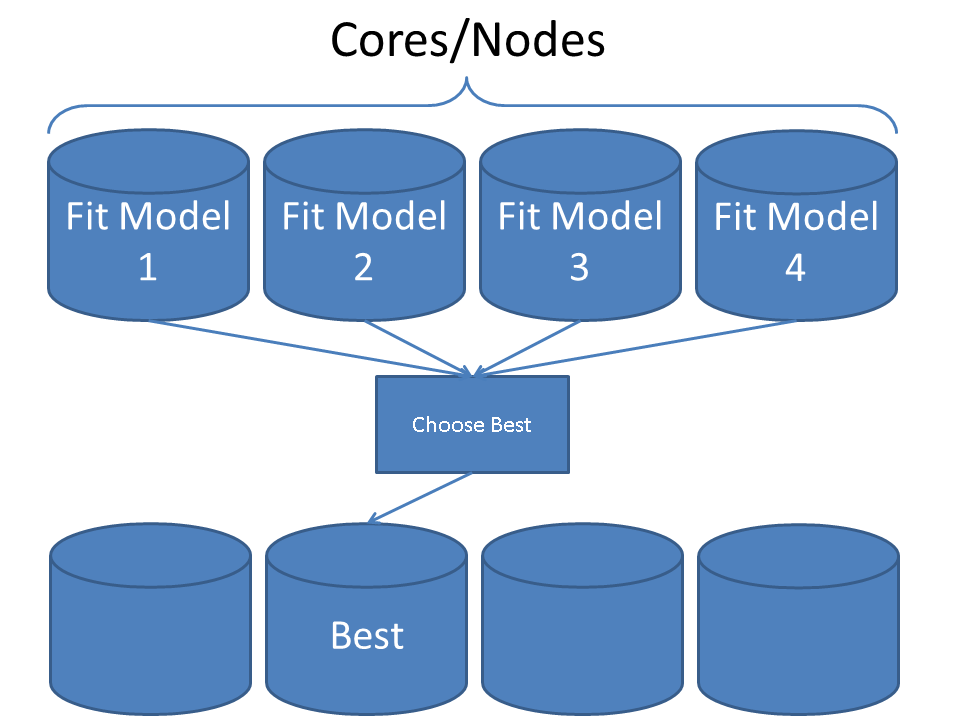
\includegraphics[width=.975\textwidth]{pics/parallelism_task}
      \end{center}
      \end{block}
    \end{minipage}
    \end{center}
  \end{block}
\end{frame}




% \subsection{Common Terminology}


\begin{frame}
  \begin{block}{Difficulty}
  \begin{enumerate}[<+-|alert@+>]
    \item \emph{Implicit parallelism}:  Parallel details hidden from user
    \item \emph{Explicit parallelism}:  Some assembly required\dots
    \item \emph{Embarrassingly Parallel}:  Also called \emph{loosely coupled}.  Obvious how to make parallel; lots of independence in computations.
    \item \emph{Tightly Coupled}:  Opposite of embarrassingly parallel; lots of dependence in computations.
  \end{enumerate}  
  \end{block}
\end{frame}

\begin{frame}
  \begin{block}{Scalability}
   \emph{Scalability}:  unitless measure of performance;
  \begin{align*}
    \frac{\tau_i}{\tau_0}
  \end{align*}
  \end{block}
\end{frame}

\begin{frame}
  \begin{block}{Types of Scalability:  Strong and Weak}
   \begin{center}
    \begin{minipage}{.475\textwidth}
    \begin{block}{Strong}
      Fix \emph{total} data size
      \centering
      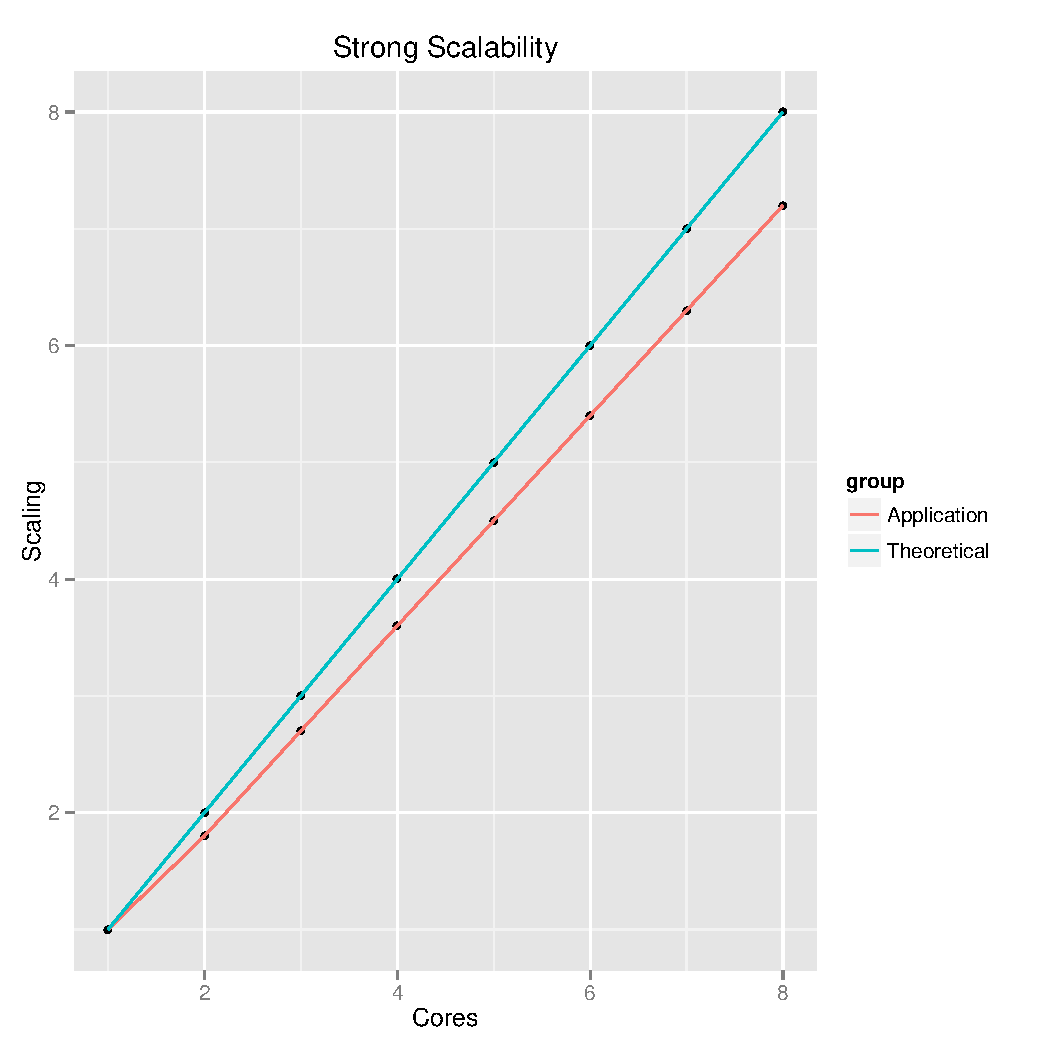
\includegraphics[width=.95\textwidth]{pics/scale_strong}
    \end{block}
    \end{minipage}
    \hspace{.1cm}
    \begin{minipage}{.475\textwidth}
    \begin{block}{Weak}
      Fix \emph{local} data size
      \centering
      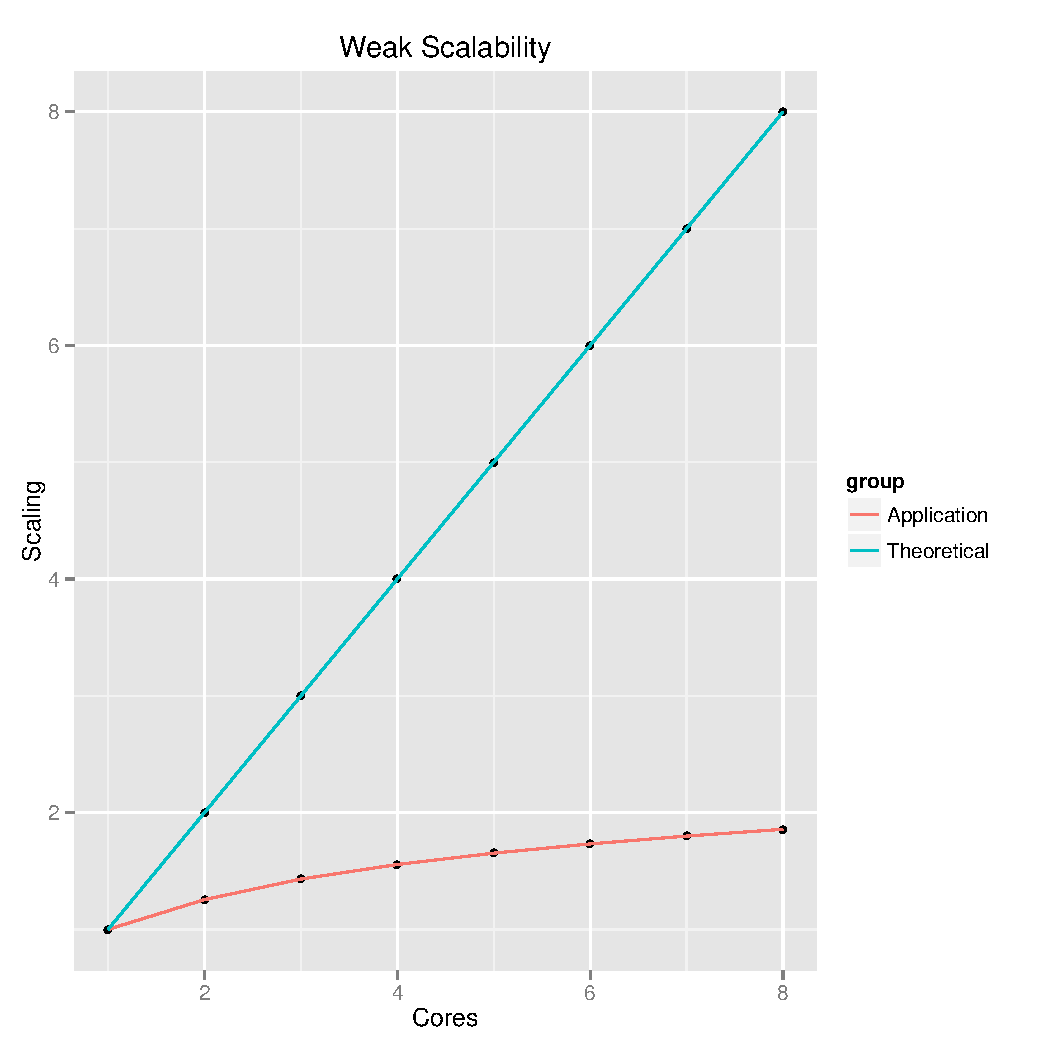
\includegraphics[width=.95\textwidth]{pics/scale_weak}
    \end{block}
    \end{minipage}
    \end{center}
    \end{block}
\end{frame}




\begin{frame}
  \begin{block}{Shared and Distributed Memory Machines}
   \begin{center}
    \begin{minipage}{.475\textwidth}
    \begin{block}{Shared Memory}
    Different processors can directly access and modify each others' memory.  There is only one node.
      \begin{center}
      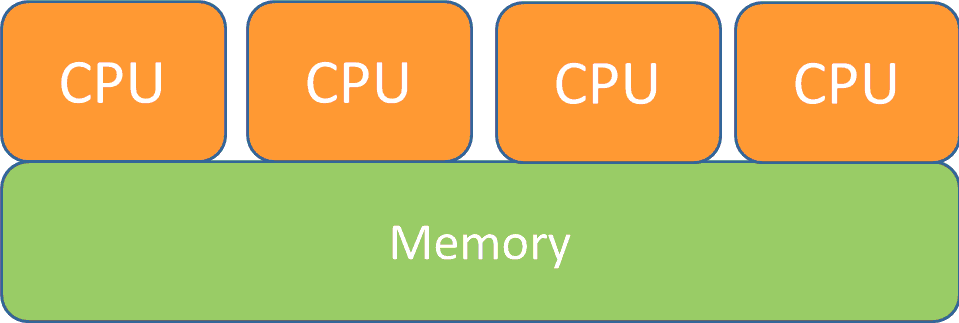
\includegraphics[width=.95\textwidth]{pics/arch_shared}
      \end{center}
      \vspace{.4cm} \ 
    \end{block}
    \end{minipage}
    \hspace{.1cm}
    \begin{minipage}{.475\textwidth}
    \begin{block}{Distributed}
    Different processors/nodes can not directly access/modify different processors'/nodes' memory.
      \begin{center}
      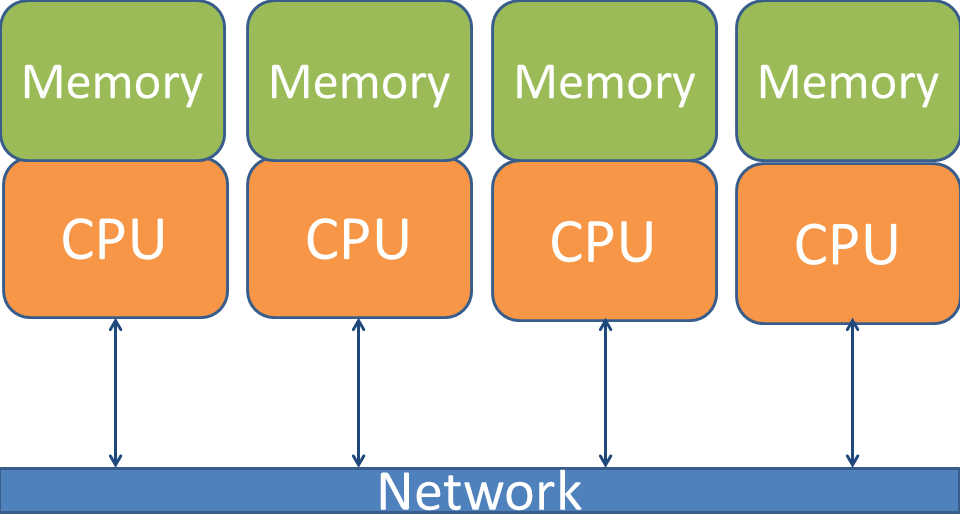
\includegraphics[width=.95\textwidth]{pics/arch_distributed}
      \end{center}
    \end{block}
    \end{minipage}
    \end{center}
    \end{block}
\end{frame}


\begin{frame}
  \begin{block}{Shared and Distributed Memory Machines}
   \begin{center}
    \begin{minipage}[t]{.47\textwidth}
    \begin{block}{Shared Memory Machines}
    \begin{center}
    Thousands of cores\\[.2cm]
    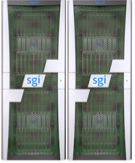
\includegraphics[scale=.65]{pics/nautilus}\\
    {\tiny \emph{Nautilus}, University of Tennessee\\1024 cores}
    \end{center}
    \end{block}
    \end{minipage}
    \hspace{.1cm}
    \begin{minipage}[t]{.47\textwidth}
    \begin{block}{Distributed Memory Machines}
    \begin{center}
    Hundreds of thousands of cores\\[.2cm]
    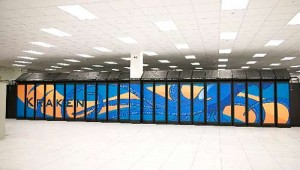
\includegraphics[width=.95\textwidth]{pics/kraken}\\
    {\tiny \emph{Kraken}, University of Tennessee\\ 112,896 cores}
    \end{center}
    \end{block}
    \end{minipage}
    \end{center}
    \end{block}
\end{frame}




\subsection{R and Parallelism}


\begin{frame}
%  \addtocounter{framenumber}{-1}
  \begin{block}{R and Parallelism}\pause
  What about R?
  \end{block}
\end{frame}

\begin{frame}
%  \addtocounter{framenumber}{-1}
  \begin{block}{Problems with Serial R}\pause
  \begin{enumerate}[<+-|alert@+>]
    \item Slow.
    \item If you don't know what you're doing, it's \emph{really} slow.
    \item Performance improvements usually for small machines.
    \item Very ram intensive.
    \item Chokes on big data.
  \end{enumerate}
  \end{block}
\end{frame}


\begin{frame}
  \begin{block}{Parallel R Packages}
   \begin{center}
    \begin{minipage}{.45\textwidth}
    \begin{block}{Shared Memory}
      \begin{enumerate}[<+-|alert@+>]
        \item \pkg{foreach}
        \item \pkg{parallel}
        \item \pkg{snow}
        \item \pkg{multicore}
      \end{enumerate}
    \end{block}
    \end{minipage}
    \hspace{.2cm}
    \begin{minipage}{.45\textwidth}
    \begin{block}{Distributed}
      \begin{enumerate}[<+-|alert@+>]
        \item \pkg{Rmpi}
        \item R+Hadoop
        \item \pkg{pbdR}
      \end{enumerate}
    \end{block}
    \end{minipage}
    \end{center}
    \end{block}
\end{frame}



\begin{frame}[shrink]
  \begin{block}{R and Parallelism}
    The solution to many of R's problems is parallelism.  However \dots\vspace{-.4cm}
   \begin{center}
    \begin{minipage}[t]{.95\textwidth}
    \begin{block}{\centering What we have}
      \begin{enumerate}[<+-|alert@+>]
        \item Mostly serial.
        \item Mostly not distributed
        \item Data parallelism mostly explicit
      \end{enumerate}
    \end{block}
    \end{minipage}
    \\\pause
    \begin{minipage}[t]{.95\textwidth}
    \begin{block}{\centering What we want}
      \begin{enumerate}[<+-|alert@+>]
        \item Mostly parallel.
        \item Mostly distributed.
        \item Mostly implicit.
      \end{enumerate}
    \end{block}
    \end{minipage}
    \end{center}
    \end{block}
\end{frame}


\begin{frame}
  \begin{block}{Why We Need Parallelism}\pause
    \begin{enumerate}[<+-|alert@+>]
      \item Saves time (long term).
      \item Data size is skyrocketing.
      \item Necessary for many problems.
      \item Like it or not, it's coming.
      \item \emph{It's really cool.}
  \end{enumerate}
  \end{block}
\end{frame}

